%%%%%%%%%%%%%%%%%%%%%%%%%%%%%%%%
% Chap 4. Constrained Optimization-Based Neuro-Adaptive Control (CoNAC) for Uncertain Euler–Lagrange Systems Under Weight and Input Constraints
%%%%%%%%%%%%%%%%%%%%%%%%%%%%%%%%

\chapter{
    CoNAC for Uncertain Euler–Lagrange Systems Under Weight and Input Constraints
} \label{chapter4}

%%%%%%%%%%%%%%%%%%%%%%%%%%%%%%%%
\section{Introduction}
%%%%%%%%%%%%%%%%%%%%%%%%%%%%%%%%

In this chapter, the constrained optimization-based neuro-adaptive controller (\allowbreak{CoNAC}) framework is extended to address the input saturation problem. 
Besides the boundedness of neural network (NN) weights, the other major issue is satisfying input constraints, particularly in systems where actuators are subject to physical limitations \cite{RN24}.
The unpredictable outputs of NNs can sometimes lead to excessively large control inputs which may destroy the actuators or the system itself. 
This problem is exacerbated in neuro-adaptive controllers (NACs) that attempt to cancel out system dynamics using conventional methods like feedback linearization or backstepping. 
In such cases, controllers may produce overly aggressive control inputs, even when the system’s natural dynamics are stabilizing, leading to unnecessary saturation of the control inputs.
The control input saturation is reformulated into convex input constraints, then incorporated into the CoNAC. 
In addition, CoNAC presented in Chapter \ref{chapter3}, is extended by substituting the single hidden layer neural network (SHLNN) by deep neural network (DNN).

%%%%%%%%%%%%%%%%%%%%%%%%%%%%%%%%
\section{Problem formulation} \label{chap4:problem}
%%%%%%%%%%%%%%%%%%%%%%%%%%%%%%%%

Consider an uncertain Euler-Lagrange system modeled as
\begin{equation}
    M(q)\ddot q + C(q,\dot q)\dot q + G(q) + F(q) = h(\tau)
    \label{chap4:eq:sys1}
\end{equation}
where $q\in \R^n$ denotes the generalized coordinate, and $\tau\in\R^n$ denotes the control input. 
The terms $M(q)\in\R^{n\times n}$, $C(q,\dot q)\in\R^{n\times n}$, and $G(q)\in\R^{n}$ represent the unknown system function matrices, while $F(q)\in\R^{n}$ denotes the external force. 
The function $h(\cdot)\in \R^n$ is a control input saturation function, where each element represents the control input saturation for each element of $\tau$. 
The gradient of $h(\cdot)$ with respect to $\tau$ is continuous and bounded, \ie $\Vert\partial h/\partial \tau\Vert_F\in L_\infty$. 

The control input saturation function represents the inherent physical limitations of the actuators. 
To account for these limitations, it is essential to incorporate physically motivated constraints into the controller design. 
Section \ref{chap4:sec:cstr_candidates} introduces candidate constraints that can be applied to ensure compliance with these physical limitations.

Using user-designed nominal system matrices $M_0 > 0$, $C_0$, and $G_0$, \eqref{chap4:eq:sys1} can be reformulated as
\begin{equation}
    M_0\ddot q+C_0\dot q+G_0 = h(\tau) + f(q,\dot q,\ddot q)
    \label{chap4:eq:sys2}
\end{equation}
where $f(q,\dot q,\ddot q) \triangleq -\Delta M(q)\ddot q-\Delta C(q,\dot q)\dot q -\Delta G(q) -F(q)\in\R^n$ is the lumped system uncertainty function. Here, $\Delta M(q)\triangleq M(q)-M_0$, $\Delta C(q,\dot q)\triangleq C(q,\dot q)-C_0$, and $\Delta G(q)\triangleq G(q)-G_0$. 

The function $f$ acts like an external disturbance, leading to a poor performance index and potential instability. 
%Therefore, an adaptive control approach is required to improve the control performance. 
The control objective is to develop a neuro-adaptive controller that enables $q$ to track a continuously differentiable desired trajectory ${q_d}(t): \R \to \R^n$, compensating for the unknown function $f$ while addressing the imposed constraints (\eg weight boundedness and input saturation).

%%%%%%%%%%%%%%%%%%%%%%%%%%%%%%%%
\section{Existing Works to Prevent Input Saturation} 
%%%%%%%%%%%%%%%%%%%%%%%%%%%%%%%%

To address input saturation, one may consider the projection operator in Section \ref{chap3:sec:proj} as one of solutions.
However, the projection operator can not be simply applied since the NNs are highly nonlinear and non-convex function.
Note that the operator is used to project adaptation direction on given convex set.

On the other hand, many studies introduced auxiliary systems. 
These systems mitigated the effects of control input saturation by modifying the control strategy when saturation occurred. 
For instance, in \cite{RN60, RN95, RN46}, auxiliary states were generated whenever input saturation was detected, and the auxiliary states were incorporated into the adaptation law to adjust the NN weights accordingly. 
For details, the auxiliary systems are generally designed as
\begin{equation}
    \dot\zeta = A_\zeta \zeta + B_\zeta \Delta\tau
\end{equation}
where $\zeta$ is the auxiliary state, $A_\zeta$ is Hurwitz matrix, $B_\zeta$ is control gain matrix, and $\Delta\tau_{(i)}=\tau_{(i)}-\tau_{\text{sat},(i)}$ is saturated control input of each control channel where $\tau_{\text{sat},(i)}$ denotes maximum or minimum value of $\tau_{(i)}$.
Thus, the auxiliary state $\zeta$ is generated when the control input $\tau$ exceeds the saturation limit $\tau_{\text{sat}}$.
Using the auxiliary state, the feedback signal for the adaptation law is modified as
\begin{equation}
    \dot{\hat\theta} = \gamma(\xi) 
    \ \to \ 
    \dot{\hat\theta}=\gamma(\xi+\zeta)
\end{equation}
where $\gamma(\cdot)$ denotes arbitrary adaptation law and $\xi$ denotes tracking error which is typically used as feedback signal for adaptation process for NACs.  
This approach helps the controller reduce input saturation by indirectly regulating the auxiliary states.
Alternatively, auxiliary states can also be used as feedback terms in the control law to directly compensate for the effects of input saturation constraints, as demonstrated in \cite{RN89, RN88, RN82}. 
In addition, the NN was used to approximate the desired control input, which compensate for input saturation in \cite{RN18}. 

However, these approaches typically handle input bound constraints on a per-input basis, and may not account for more complex and nonlinear constraints, like input norm constraints, which are commonly found in physical systems such as robotic actuators or motor systems due to their power limitations.

%%%%%%%%%%%%%%%%%%%%%%%%%%%%%%%%
\section{CoNAC with Weight and Input Constraints}
%%%%%%%%%%%%%%%%%%%%%%%%%%%%%%%%

The architecture of the proposed CoNAC is illustrated in Fig.~\ref{chap4:fig:ctrl}, consisting of: a reference generator, a DNN that functions as NAC, and a weight optimizer for the DNN. 
The simple version of the CoNAC is introduced in Chapter \ref{chapter3} ahead with the SHLNN instead of the DNN and the weight norm constraints.
We will extend it to the DNN with the weight and input constraints in this chapter.

\begin{figure*}[t]
    \centering
    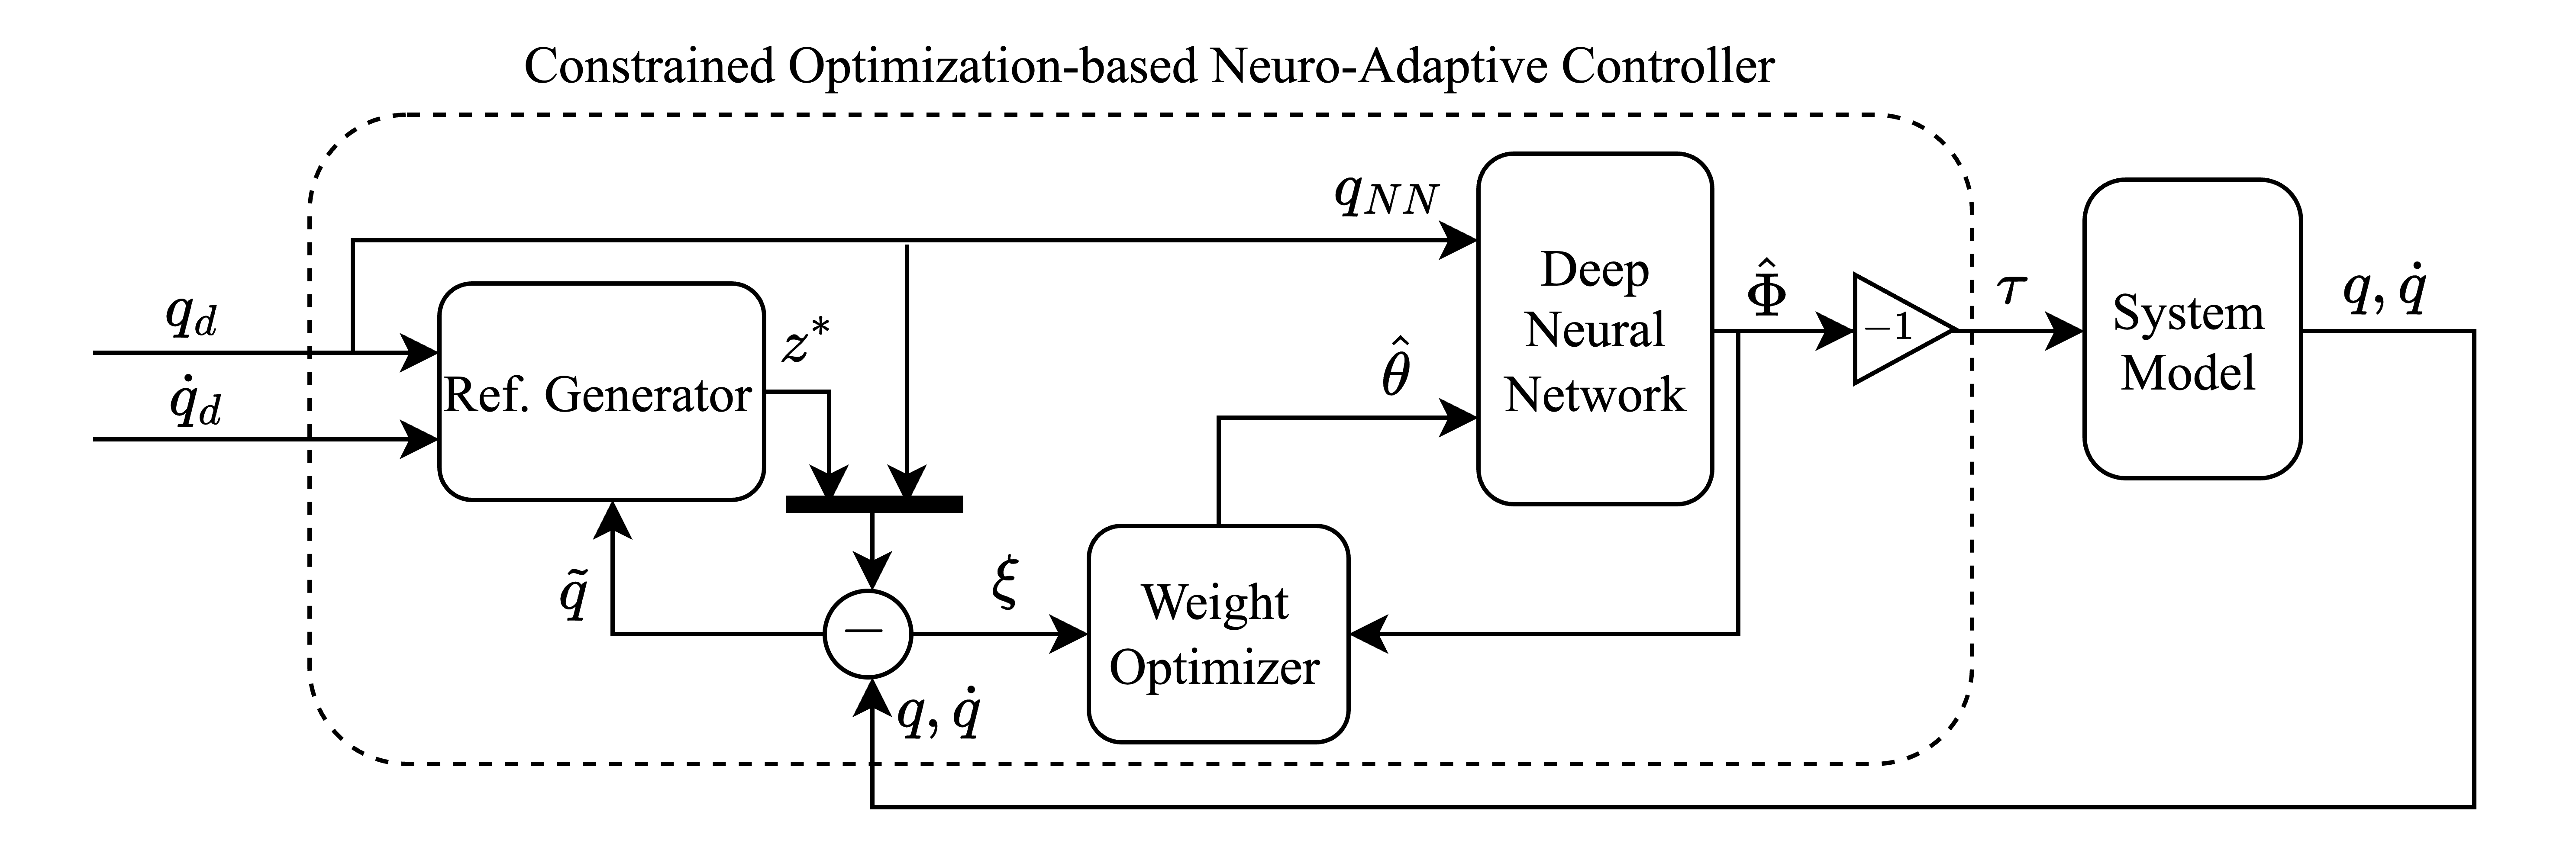
\includegraphics[width=0.9\linewidth]{imgs/ControllerChap4.drawio.png}
    \caption{Architecture of the constrained optimization-based neuro-adaptive controller (CoNAC).}
    \label{chap4:fig:ctrl}
\end{figure*}

\subsection{Control Law Development}

The system dynamics \eqref{chap4:eq:sys2} can be represented as
\begin{equation}
    \begin{aligned}
        \dot {q} &= {z},\\
        \dot {z} &= -M_0^{-1} C_0 {z}-M_0^{-1} G_0+M_0^{-1} h(\tau) + M_0^{-1} f,
    \end{aligned}
    \label{chap4:eq:x_dyna}
\end{equation}
where ${z}\triangleq \dot q$.

Similar to the control law development in Section \ref{chap3:sec:ctrl_dev}, the reference generator generates the desired trajectory $z^*\triangleq -k_q\tilde q+\dot q_d$ for $z\triangleq \dot q$, where $\tilde q\triangleq q-q_d$ and $k_q\in\R_{>0}$.
Then the desired stabilizing controller can be designed as
\begin{equation}
    \tau^* = -M_0(k_z\tilde z+\tilde q)+C_0 z+G_0-f+M_0\dot z^*
    \label{chap4:eq:desired_control}
\end{equation}
where $\tilde z\triangleq z-z^*$, $k_z\in\R_{>0}$, and $k_z\in\R_{>0}$.
Note that the control law $\tau^*$ cannot be realized because of $f$.

The DNN presented in Section \ref{chap2:sec:DNN}, is defined as 
\begin{equation}
    \Phi(q_{NN};\theta) \triangleq 
    \underbrace{
        V_k^T  \phi_{k}(
        \underbrace{
        V_{k-1}^T   \cdots \phi_2(
        \underbrace
            {
            V_1^T   \phi_1(
            \underbrace
            {
            V_0^T   q_{NN}
            }_{\Phi_0}
            )
        }_{\Phi_1}
        )\cdots )
        }_{\Phi_{k-1}}
        )
    }_{\Phi_k}
\end{equation}
where $q_{NN}$ denotes the NN input vector, $V_i\in\R^{(l_i+1)\times l_{i+1}}$ is the weight matrix of the $i\textsuperscript{th}$ layer, and $\phi_i: \R^{l_i}\to\R^{l_i+1}$ represents the activation function of the $i\textsuperscript{th}$ layer.
For the simplicity, the weights are vectorized in $\theta\triangleq[\theta_i]_{i\in[k,\cdots,0]}\in\R^{\Xi}$ consisting of vectorized weights of each layer such that $\theta_i\triangleq\text{vec}(V_i)\in\R^{\Xi_i}$, where $\Xi\triangleq \sum_{i\in[k,\cdots 0]}$ denotes the total number of weights and $\Xi_i\triangleq (l_i+1)l_{i+1}$ denote the number of weights in the $i\textsuperscript{th}$ layer, respectively.

According to Theorem \ref{chap2:thm:uni_approx}, the desired control law $\tau^*$ can be approximated by the DNN with the ideal weight vector $\theta^*$ on a compact subset $\Omega_{NN}\in\R^{l}$ to $\epsilon$-accuracy, such that $\sup_{q_{NN}\in\Omega_{NN}}\Vert \Phi(q_{NN};\theta^*) - \tau^* \Vert = \epsilon < \infty$.
The ideal weight $\theta^*$ is typically assumed to be bounded, \ie $\Vert\theta^*\Vert\le \bar\theta<\infty$.
In this thesis, $\theta^*$ is defined as a local optimal point, rather than a global optimal point.

Then, the desired control law can be represented as follows:
\begin{align}
    \tau^*=& -(\Phi^*+\epsilon),
\end{align}
which is estimated online by
\begin{align}
    \tau =& -\hat\Phi,
    \label{chap4:eq:approx_control}
\end{align}
where $\hat\Phi\triangleq\Phi(q_{NN};\hat\theta)$, and  $\hat\theta$ is the estimated weight vector for $\theta^*$.

Using \eqref{chap4:eq:x_dyna}, \eqref{chap4:eq:desired_control}, \eqref{chap4:eq:approx_control}, and the definition of $\tilde z$ the error dynamics can be derived as
\begin{equation}
    \begin{aligned}
        \dot {\tilde q} = & -{k_q} {\tilde q} + {\tilde z} \\
        \dot {\tilde z} = & -{\tilde q} -{k_z} {\tilde z} + M_0^{-1} (\Phi^*-h(\hat\Phi)+\epsilon).
    \end{aligned}
    \label{chap4:eq:e_dyna}
\end{equation}
The error dynamics \eqref{chap4:eq:e_dyna} can be represented as a first-order system: 
\begin{equation}
    \dot\xi = A_\xi \xi + B_\xi (\Phi^*-h(\hat\Phi)+\epsilon)
    \label{chap4:eq:xi_dyna}
\end{equation}
where 
$\xi\triangleq[{\tilde q}^T  , {\tilde z}^T  ]^T  \in\R^{2n}$ denotes the augmented error,
and
\begin{equation}
    A_\xi \triangleq 
    \begin{bmatrix}
        -{k_q} I_n &I_n\\-I_n& -{k_z} I_n
    \end{bmatrix}
    ,\ 
    B_\xi \triangleq 
    \begin{bmatrix}
        0_{n\times n}\\M_0^{-1}
    \end{bmatrix}.
\end{equation}
Note that $A_\xi$ is a stable matrix, and $\Vert B_\xi\Vert_F<\infty$.
For further sections, $\phi^*_i \triangleq\phi_i(\Phi^*_{i-1})$ and ${\phi^*}'_i = \partial \phi^*_i/\partial \Phi^*_{i-1}$, and $\hat\phi_i \triangleq\phi_i(\hat\Phi_{i-1})$ and $\hat\phi_i' = \partial \hat\phi_i/\partial \hat{\Phi}_{i-1}$.

%%%%%%%%%%%%%%%%%%%%%%%%%%%%%%%%
\subsection{Weight Adaptation Laws}
%%%%%%%%%%%%%%%%%%%%%%%%%%%%%%%%

The adaptation laws are same as the previous Section \ref{chap3:sec:weight_adap} and represented as follows:
\begin{subequations}
    \begin{align}
        \dot {\hat\theta}&=-\alpha {\partial L\over\partial \hat\theta}
        =-\alpha 
        \bigg(
        {\partial J\over \partial \hat\theta}+\sum_{j\in\mathcal{A}}
        \lambda_j {\partial c_j\over\partial \hat\theta}
        \bigg),
    \label{chap4:eq:adap_th}
        \\
        \dot\lambda_j& = \beta_j{\partial L\over\partial \lambda_j} = \beta_j c_j ,
        \quad\quad\quad\quad      \      
        \forall j\in\mathcal A,
    \label{chap4:eq:adap_L}
        \\
        \lambda_j & = \max(\lambda_j,0) ,
        \quad\quad\quad\quad\ \ \ \ \ 
        \forall j\in\mathcal A,
    \label{chap4:eq:adap_L_max}
    \end{align}
    \label{chap4:eq:adap}
\end{subequations}
where $L\triangleq J(\xi;\hat\theta)+\sum_{j\in\mathcal A}\lambda_j c_j(\hat\theta)$ denotes Lagrangian function consisting of the original objective function $J\triangleq(1/2)\xi^T\xi$, the inequality constraint $c_j,\ j\in\mathcal I$ and Lagrange multiplier $\lambda_j$, where $\mathcal I$ is the set of imposed constraints, $\mathcal A \triangleq \{j\in\mathcal I\ |\ c_j\ge 0\}$ represents the active set.
Moreover, $\alpha\in\R_{>0}$ denotes the adaptation gain (learning rate) and $\beta_j\in\R_{>0}$ denotes the update rate of the Lagrange multipliers in $\mathcal A$. 

%%%%%%%%%%%%%

As presented in Section \ref{chap3:sec:weight_adap}, the gradient of the objective function with respect to the weights can be represented as
\begin{equation}
    {\partial J\over\partial \hat\theta}
    =
    \begin{bmatrix}
        \partial J/\partial\hat\theta_k\\\vdots\\\partial J/\partial\hat\theta_0\\
    \end{bmatrix}
    =
    {\partial \xi\over\partial \hat\theta}^TW
    {\partial \xi\over\partial \hat\theta}
\end{equation}
where $W\in\R^{2n\times 2n}$ is a positive weight matrix, and $\partial \xi/\partial \hat\theta$ is the sensitivity of the weights to the augmented error.
The sensitivity of the weights can be obtained by simulating the sensitivity equation as follows:
\begin{equation}
    \begin{aligned}
        \dot \eta&= 
        \begin{bmatrix}
            \eta_k&
            \eta_{k-1}&
            \cdots &
            \eta_0
        \end{bmatrix}'
        \\
        &=A_\xi
        \begin{bmatrix}
            \eta_k&
            \cdots &
            \eta_0
        \end{bmatrix}
        -B_\xi{\partial h\over\partial \tau}
        \begin{bmatrix}
            (I_{l_{k+1}}\otimes \hat\phi_{k}^T  )&
        \cdots&
        (\cdot)
        \end{bmatrix}
    \end{aligned}
    \label{chap4:eq:eta_dyna}
\end{equation}
with zero initial value of $\eta$, since the initial $\xi$ is independent of the weights.

The adaptation is implemented using Algorithm \ref{chap4:alg:alg1}. 
For implementation in the discrete-time domain, it is recommended to use a sufficiently small sampling time $T_s$. 
If a large $T_s$ is used, $\alpha$ and $\beta_j$ should satisfy the Armijo condition \cite[Chap.~3 eq.~(3.4)]{RN9} to ensure that the objective function decreases.

\begin{algorithm}[t]
    \caption{Weight optimizer implementation.}\label{chap4:alg:alg1}
    \SetKwInOut{Input}{input}
    \SetKwInOut{Output}{output}
        \Input{$\xi$, $\hat\theta$, $\lambda_j$, $\eta$}
        \Output{$\hat\theta$, $\lambda_j$, $\eta$}
        \BlankLine
        \emph{Set $\mathcal A \leftarrow \mathcal A\cup \{j\}$ for all $c_j\ge0$}\;
        \emph{Determine update matrix $\dot\eta$ using \eqref{chap4:eq:eta_dyna}}\;
        \emph{Update $\eta\leftarrow \eta +\dot\eta\cdot T_s$}\; 
        \emph{Determine update directions $\dot{\hat\theta}$, $[\dot\lambda_j]_{j\in\mathcal A}$ using \eqref{chap4:eq:adap_th}, \eqref{chap4:eq:adap_L}}\;
        \emph{Update weight vector $\hat\theta\leftarrow \hat\theta+\dot{\hat\theta}\cdot T_s$}\;
        \emph{Update multipliers $[\lambda_j]_{j\in\mathcal A}\leftarrow [\lambda_j]_{j\in\mathcal A}+[\dot\lambda_j]_{j\in\mathcal A}\cdot T_s$}\;
        \emph{$[\lambda_j]_{j\in\mathcal A}\leftarrow \max([\lambda_j]_{j\in\mathcal A}, 0)$}\;
        \emph{Set $\mathcal A \leftarrow \mathcal A - \{j\}$ for all $\lambda_j=0$}\;
\end{algorithm}

%%%%%%%%%%%%%%%%%%%%%%%%%%%%%%%%
\section{Constraint Candidates} \label{chap4:sec:cstr_candidates}
%%%%%%%%%%%%%%%%%%%%%%%%%%%%%%%%

This section introduces weight and potential input constraints that can be used in the CoNAC. 
The controller can handle any combination of the following constraints, provided they meet the specified assumptions.

\begin{assumption}
    The constraint functions $c_j(\hat\theta),\ \forall j\in\mathcal I$ are convex in the $\tau$-space and satisfy $c_j(0) \le 0$ and $c_j(\theta^*)\le 0$.
    \label{chap4:assum:assum1}
\end{assumption}

\begin{assumption}
    The selected constraints satisfy the Linear Independence Constraint Qualification (LICQ) defined in Definition \ref{chap2:def:LICQ}.
    \label{chap4:assum:assum2}
\end{assumption}

\subsection{Weight Norm Constraint} \label{chap4:sec:weight_cstr}

\begin{figure*}[t]
    \centering
    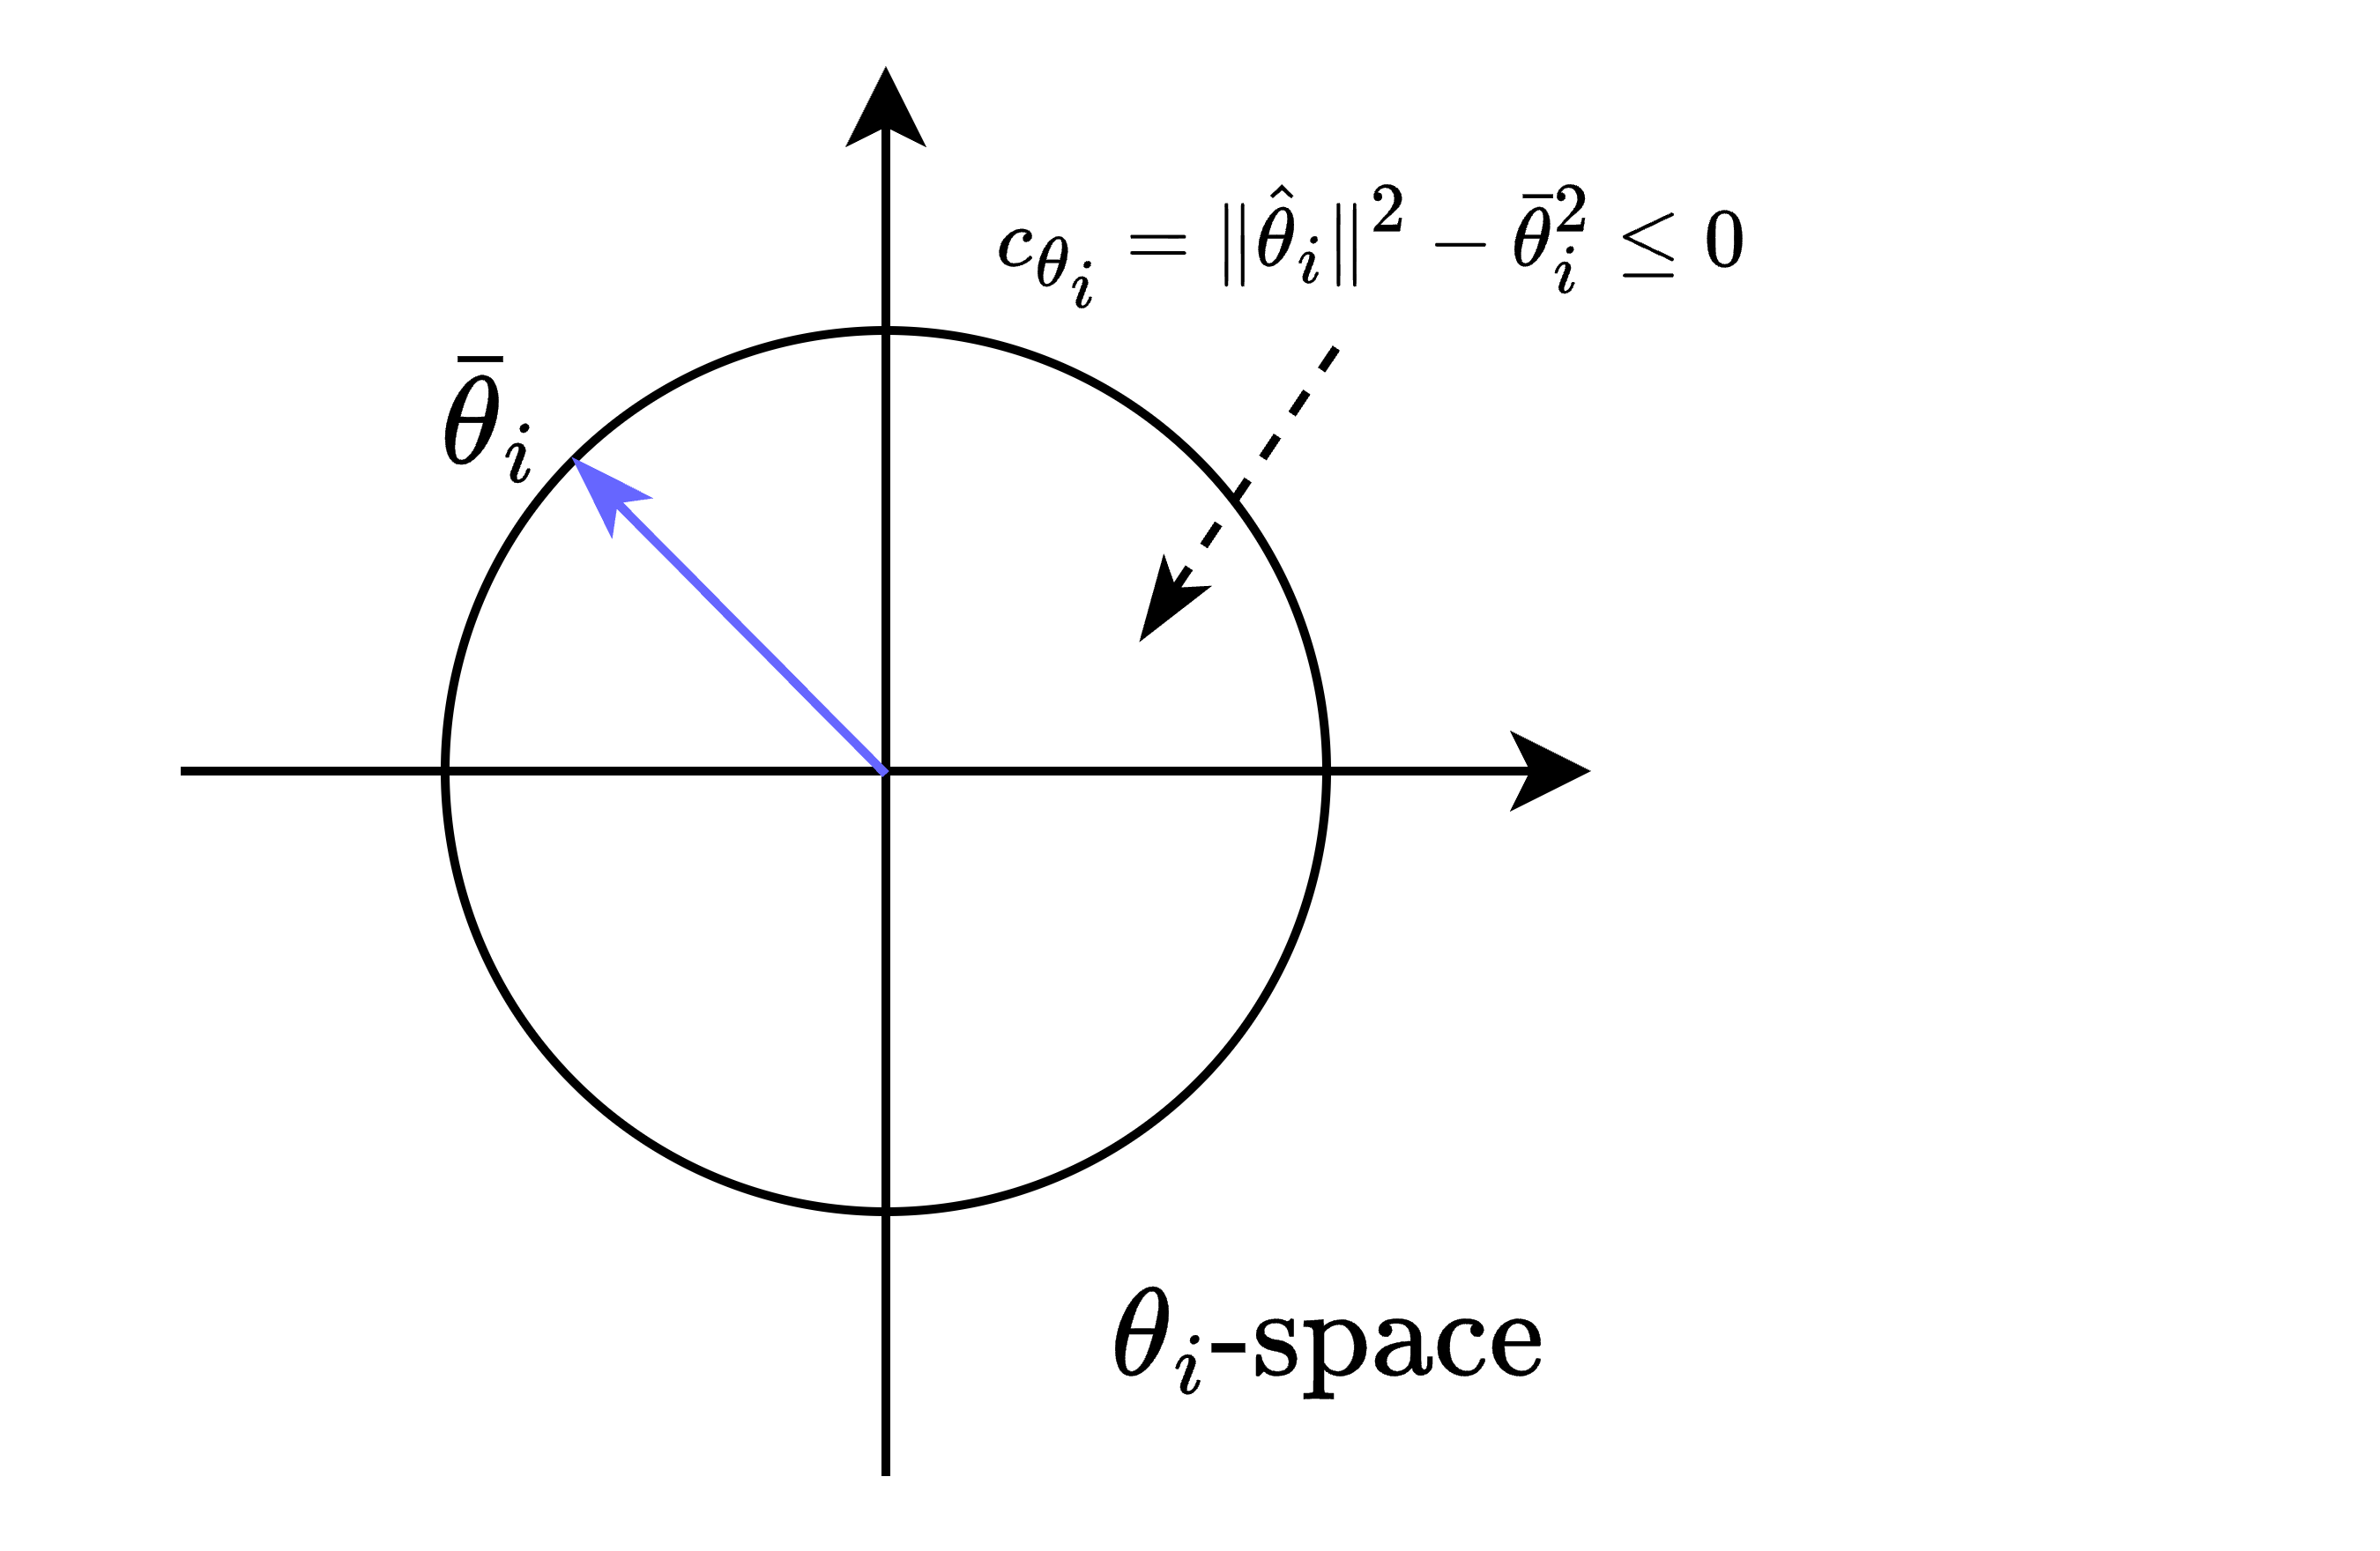
\includegraphics[width=0.5\linewidth]{imgs/cstr_weight.drawio.png}
    \caption{Weight norm constraints.}
    \label{chap4:fig:cstr:weight}
\end{figure*}

The weight norm constraint $\mathbf{c}_{\theta}\triangleq [c_{\theta_i}]_{i\in[0,\cdots ,k]}\in\R^{k+1}$ limits the maximum norm of each layer's weight vector as shown in Fig.~\ref{chap4:fig:cstr:weight}, where
\begin{equation}
    c_{\theta_i}=\Vert \hat\theta_i\Vert^2 -\bar\theta_i^2 \le 0
    \label{chap4:eq:cstr:weight}
\end{equation}
with $\bar\theta_i<\infty$ denoting the maximum allowable norm for $\hat\theta_i$. 
The gradient of $\mathbf{c}_\theta$ with respect to $\hat\theta$ is given by
\begin{equation}
    {\partial \mathbf c_\theta \over \partial \hat\theta}
    \triangleq
    \begin{bmatrix}
        (\partial c_{\theta_0}/\partial \hat\theta)^T
        \\ 
        \vdots 
        \\
        (\partial c_{\theta_k}/\partial \hat\theta)^T
    \end{bmatrix}
    = 2\cdot 
    \begin{bmatrix}
        0&0&\cdots & \hat\theta_0^T\\
        \vdots&\vdots&\ddots&\vdots\\
        0&\hat\theta^T_{k-1}&\cdots &0\\
        \hat\theta^T_k&0&\cdots &0
    \end{bmatrix}
    \in\R^{(k+1)\times\Xi}
    .
    \label{chap4:eq:cstr:weight_grad}
\end{equation}

%\begin{remark} Imposing the weight norm constraint is analogous to applying $L_2$-regularization, a common technique used in DNN training to prevent parameter drift or overfitting \cite{RN23}, by minimizing the $L_2$ norm of the estimated weight vector $\hat\theta$. Typically, $L_2$-regularization adds a term $\lambda\Vert\hat\theta\Vert_2^2$ to the objective function $J$, where $\lambda\in\R_{>0}$ is a constant $L_2$ coefficient. This term biases the trainable weights $\hat\theta$ toward the origin (\ie $\hat\theta = 0$) in the adaptation law \eqref{eq. adaptation law th}. In contrast, within the proposed controller, the term associated with the maximum weight ball constraint in the adaptation law (\ie $\sum_{j\in\mathcal{A}}\lambda_j (\partial c_j/\partial \hat\theta)$ in \eqref{eq. adaptation law th}) vanishes when the constraint is satisfied (\ie $\lambda_j = 0$).
    % 1. 제약조건이 사라져 자유롭게 ball condition 내에서 optimal point로 접근할 수 있다.
%    As a result, $\hat\theta$ can still converge to $\theta^*$ without being restricted to the origin.
%    Moreover, $\lambda_{b_i}$ which corresponds to $\lambda$ varies as the constraint is violated, while $L_2$-regularization has a constant coefficient.
%    \label{remark: ball cstr}
%\end{remark}

\subsection{Input Bound Constraint} \label{chap4:sec:input_cstr}

\begin{figure*}[t]
    \centering
    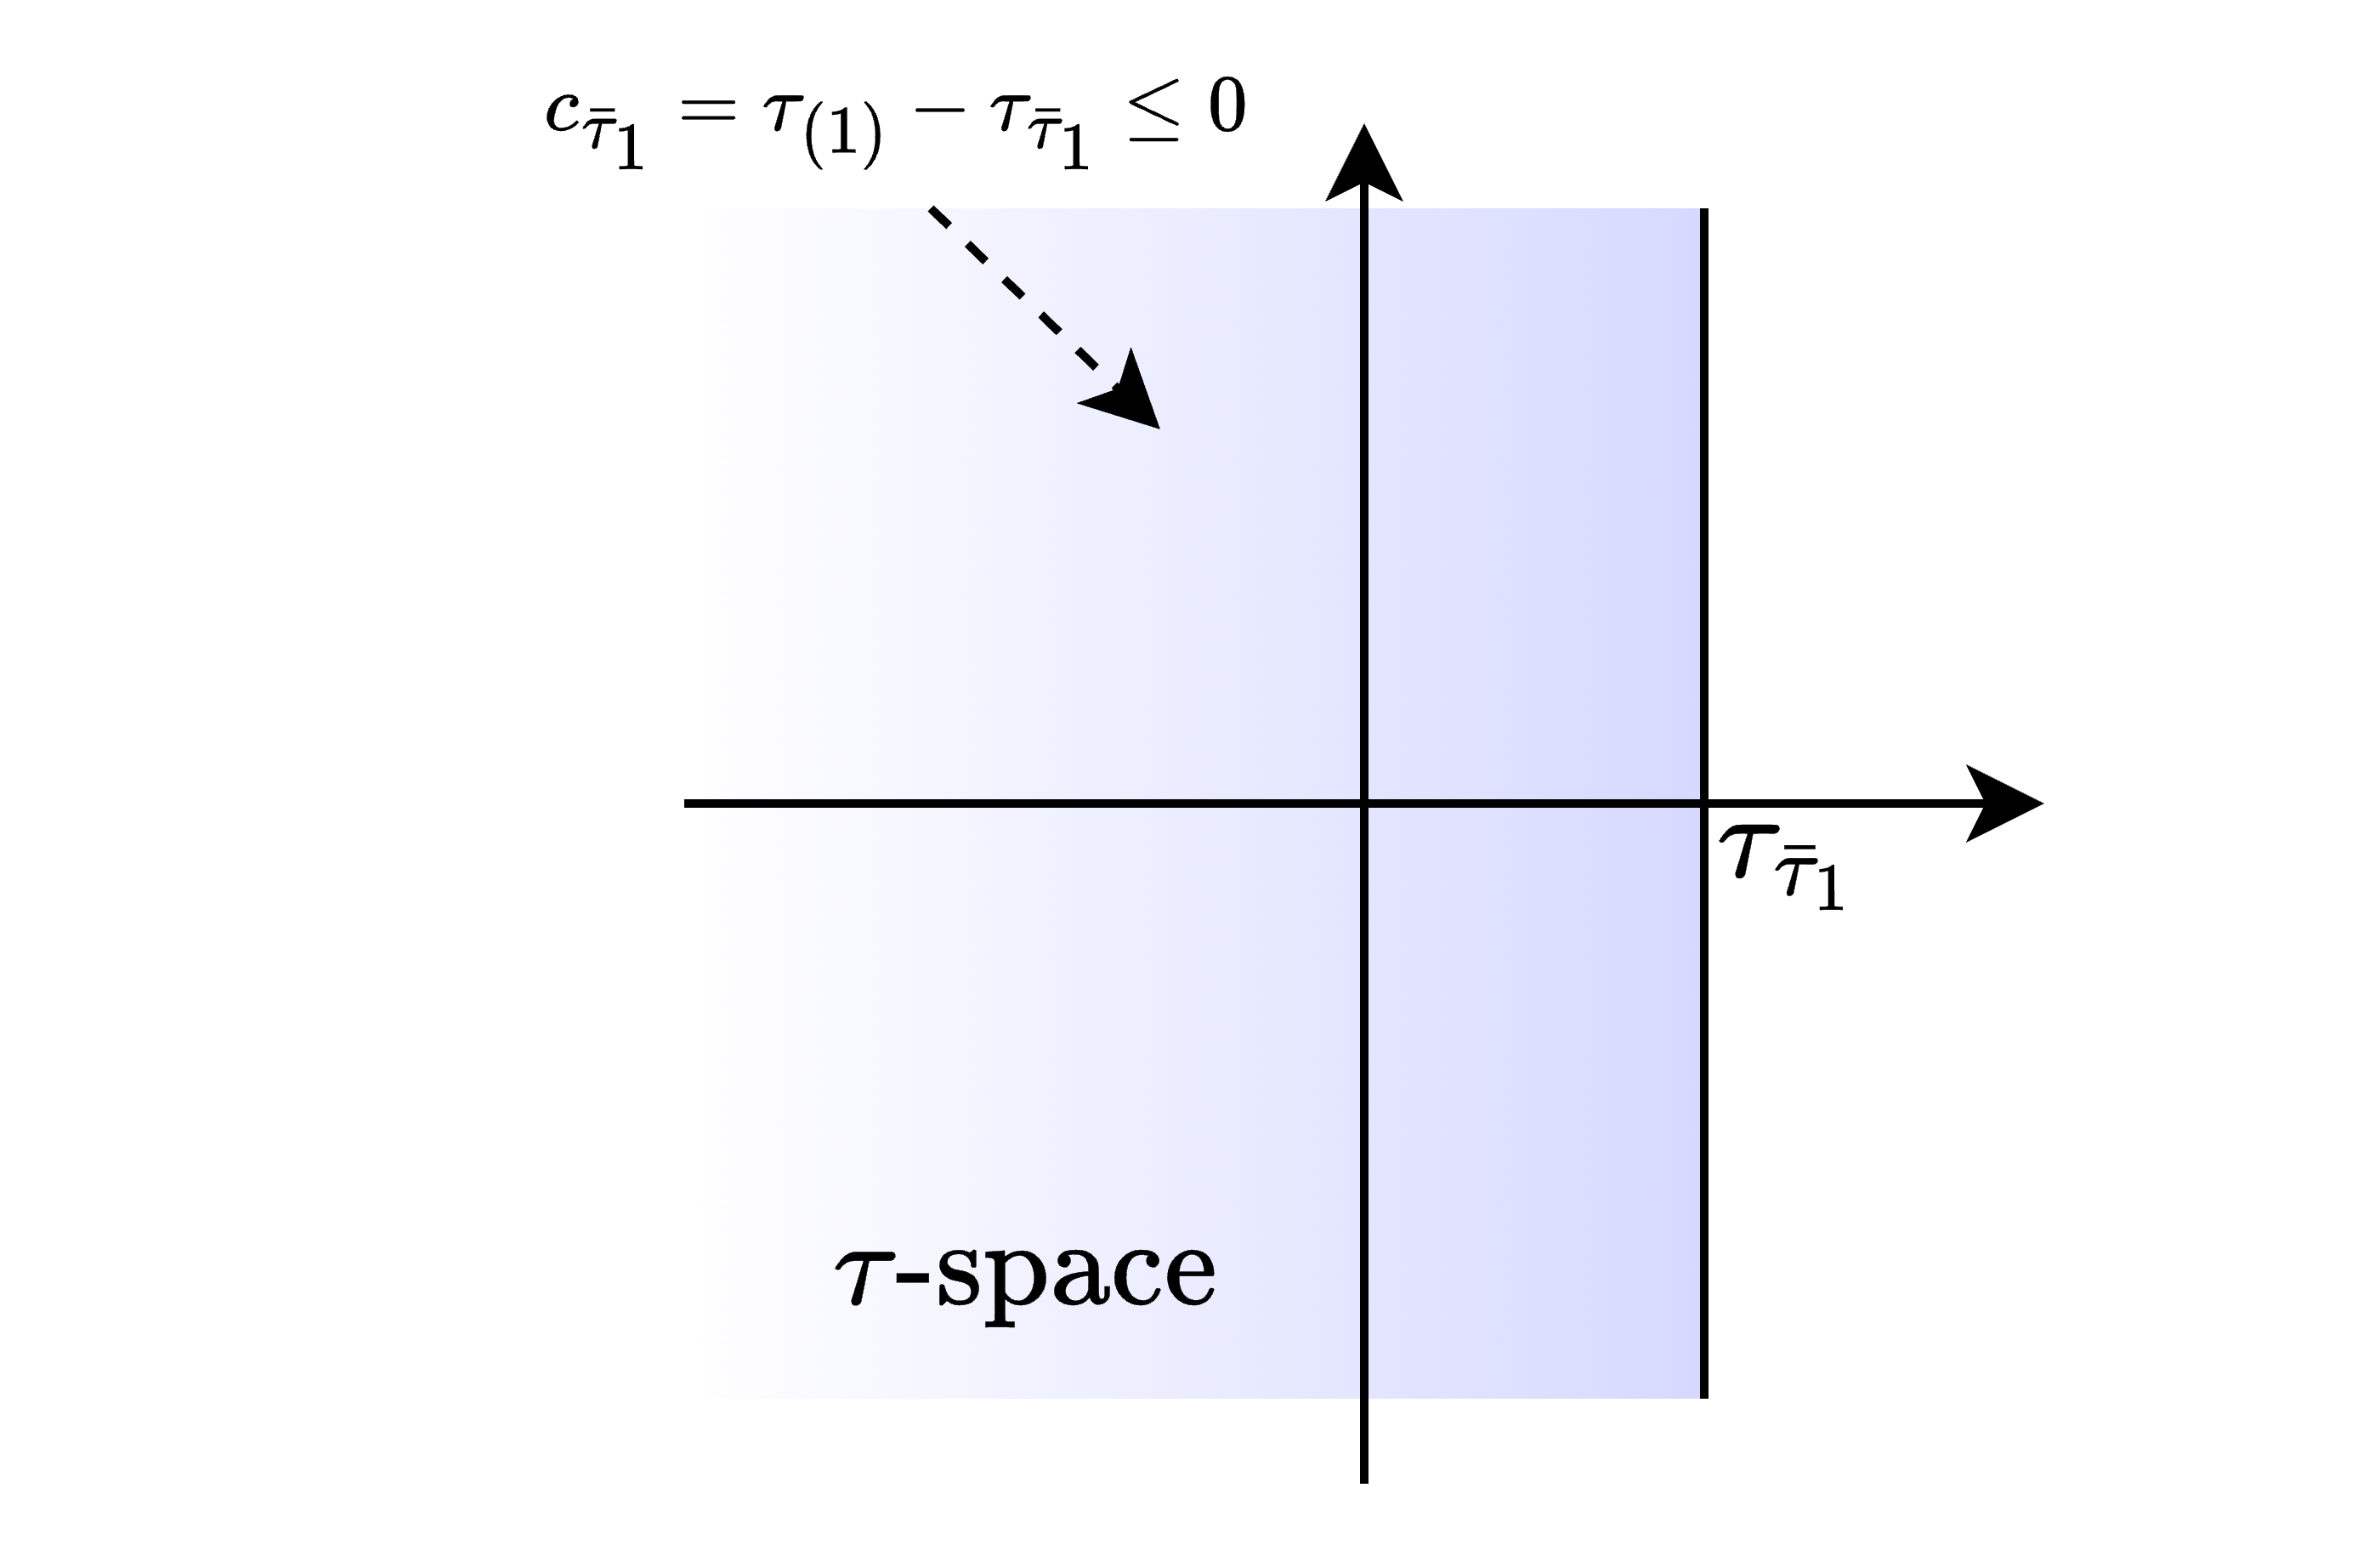
\includegraphics[width=0.5\linewidth]{imgs/cstr_input_bound.drawio.png}
    \caption{Input bound constraints.}
    \label{chap4:fig:cstr:u_bound}
\end{figure*}

Most physical systems have control input limits due to electrical and mechanical limitations. 
These are expressed as $\mathbf{c}_{\overline \tau}\triangleq [c_{\overline \tau_i}]_{i\in[1,\cdots,n]}$ and $\mathbf{c}_{\underline\tau}\triangleq [c_{\underline\tau_i}]_{i\in[1,\cdots,n]}$, where
\begin{equation}
    \begin{aligned}
        c_{\overline \tau_i}=\tau_{(i)} - {\tau_{\overline \tau_i}} \le 0
        ,\quad
        c_{\underline\tau_i}={\tau_{\underline\tau_i}}-\tau_{(i)} \le 0
    \end{aligned}
    \label{chap4:eq:cstr:input_bound}
\end{equation}
with $\tau_{\overline \tau_i}$ and $\tau_{\underline\tau_i}$ representing the maximum and minimum control input bounds, respectively.
For the case of $c_{\overline \tau_1 }$ is shown in Fig.~\ref{chap4:fig:cstr:u_bound}.
% The corresponding Lagrange multipliers are $\lambda_{u_j,i},\ \forall j\in[M,m]$. 
The gradients of $\mathbf{c}_{\overline \tau}$ and $\mathbf{c}_{\underline\tau}$ with respect to $\hat\theta$ are given by
\begin{equation}
    \begin{aligned}
        {\partial \mathbf \mathbf c_{\overline \tau} \over \partial \hat\theta}
        \triangleq
        & 
        \begin{bmatrix}
            (\partial c_{\overline \tau_1}/\partial \hat\theta)^T \\
            \vdots \\
            (\partial c_{\overline \tau_n}/\partial \hat\theta)^T
        \end{bmatrix}
         = -{\partial \hat\Phi\over\partial\hat\theta}
        =
        -\begin{bmatrix}
            (I_{l_{k+1}}\otimes \hat\phi_{k}^T)&
            % V_k^T \phi_{k}' (I_{l_{k}}\otimes  \phi_{k-1}^T)&
            \cdots &
            (
            \cdot
            )
        \end{bmatrix} 
        &
        \in
        \R^{n\times \Xi}
        , 
        \\
        {\partial \mathbf \mathbf c_{\underline\tau} \over \partial \hat\theta}         
        \triangleq
        & 
        \begin{bmatrix}
            (\partial c_{\underline\tau_1}/\partial \hat\theta)^T \\
            \vdots \\
            (\partial c_{\underline\tau_n}/\partial \hat\theta)^T
        \end{bmatrix}
        = +{\partial \hat\Phi\over\partial\hat\theta}
        =
        +\begin{bmatrix}
            (I_{l_{k+1}}\otimes \hat\phi_{k}^T)&
            % V_k^T \phi_{k}' (I_{l_{k}}\otimes  \phi_{k-1}^T)&
            \cdots &
            (
            \cdot
            )
        \end{bmatrix} 
        &
        \in
        \R^{n\times \Xi}
        .
    \end{aligned}
    \label{chap4:eq:cstr:input_bound_grad}
\end{equation}

\subsection{Input Norm Constraint} \label{chap4:sec:input_norm_cstr}

\begin{figure*}[t]
    \centering
    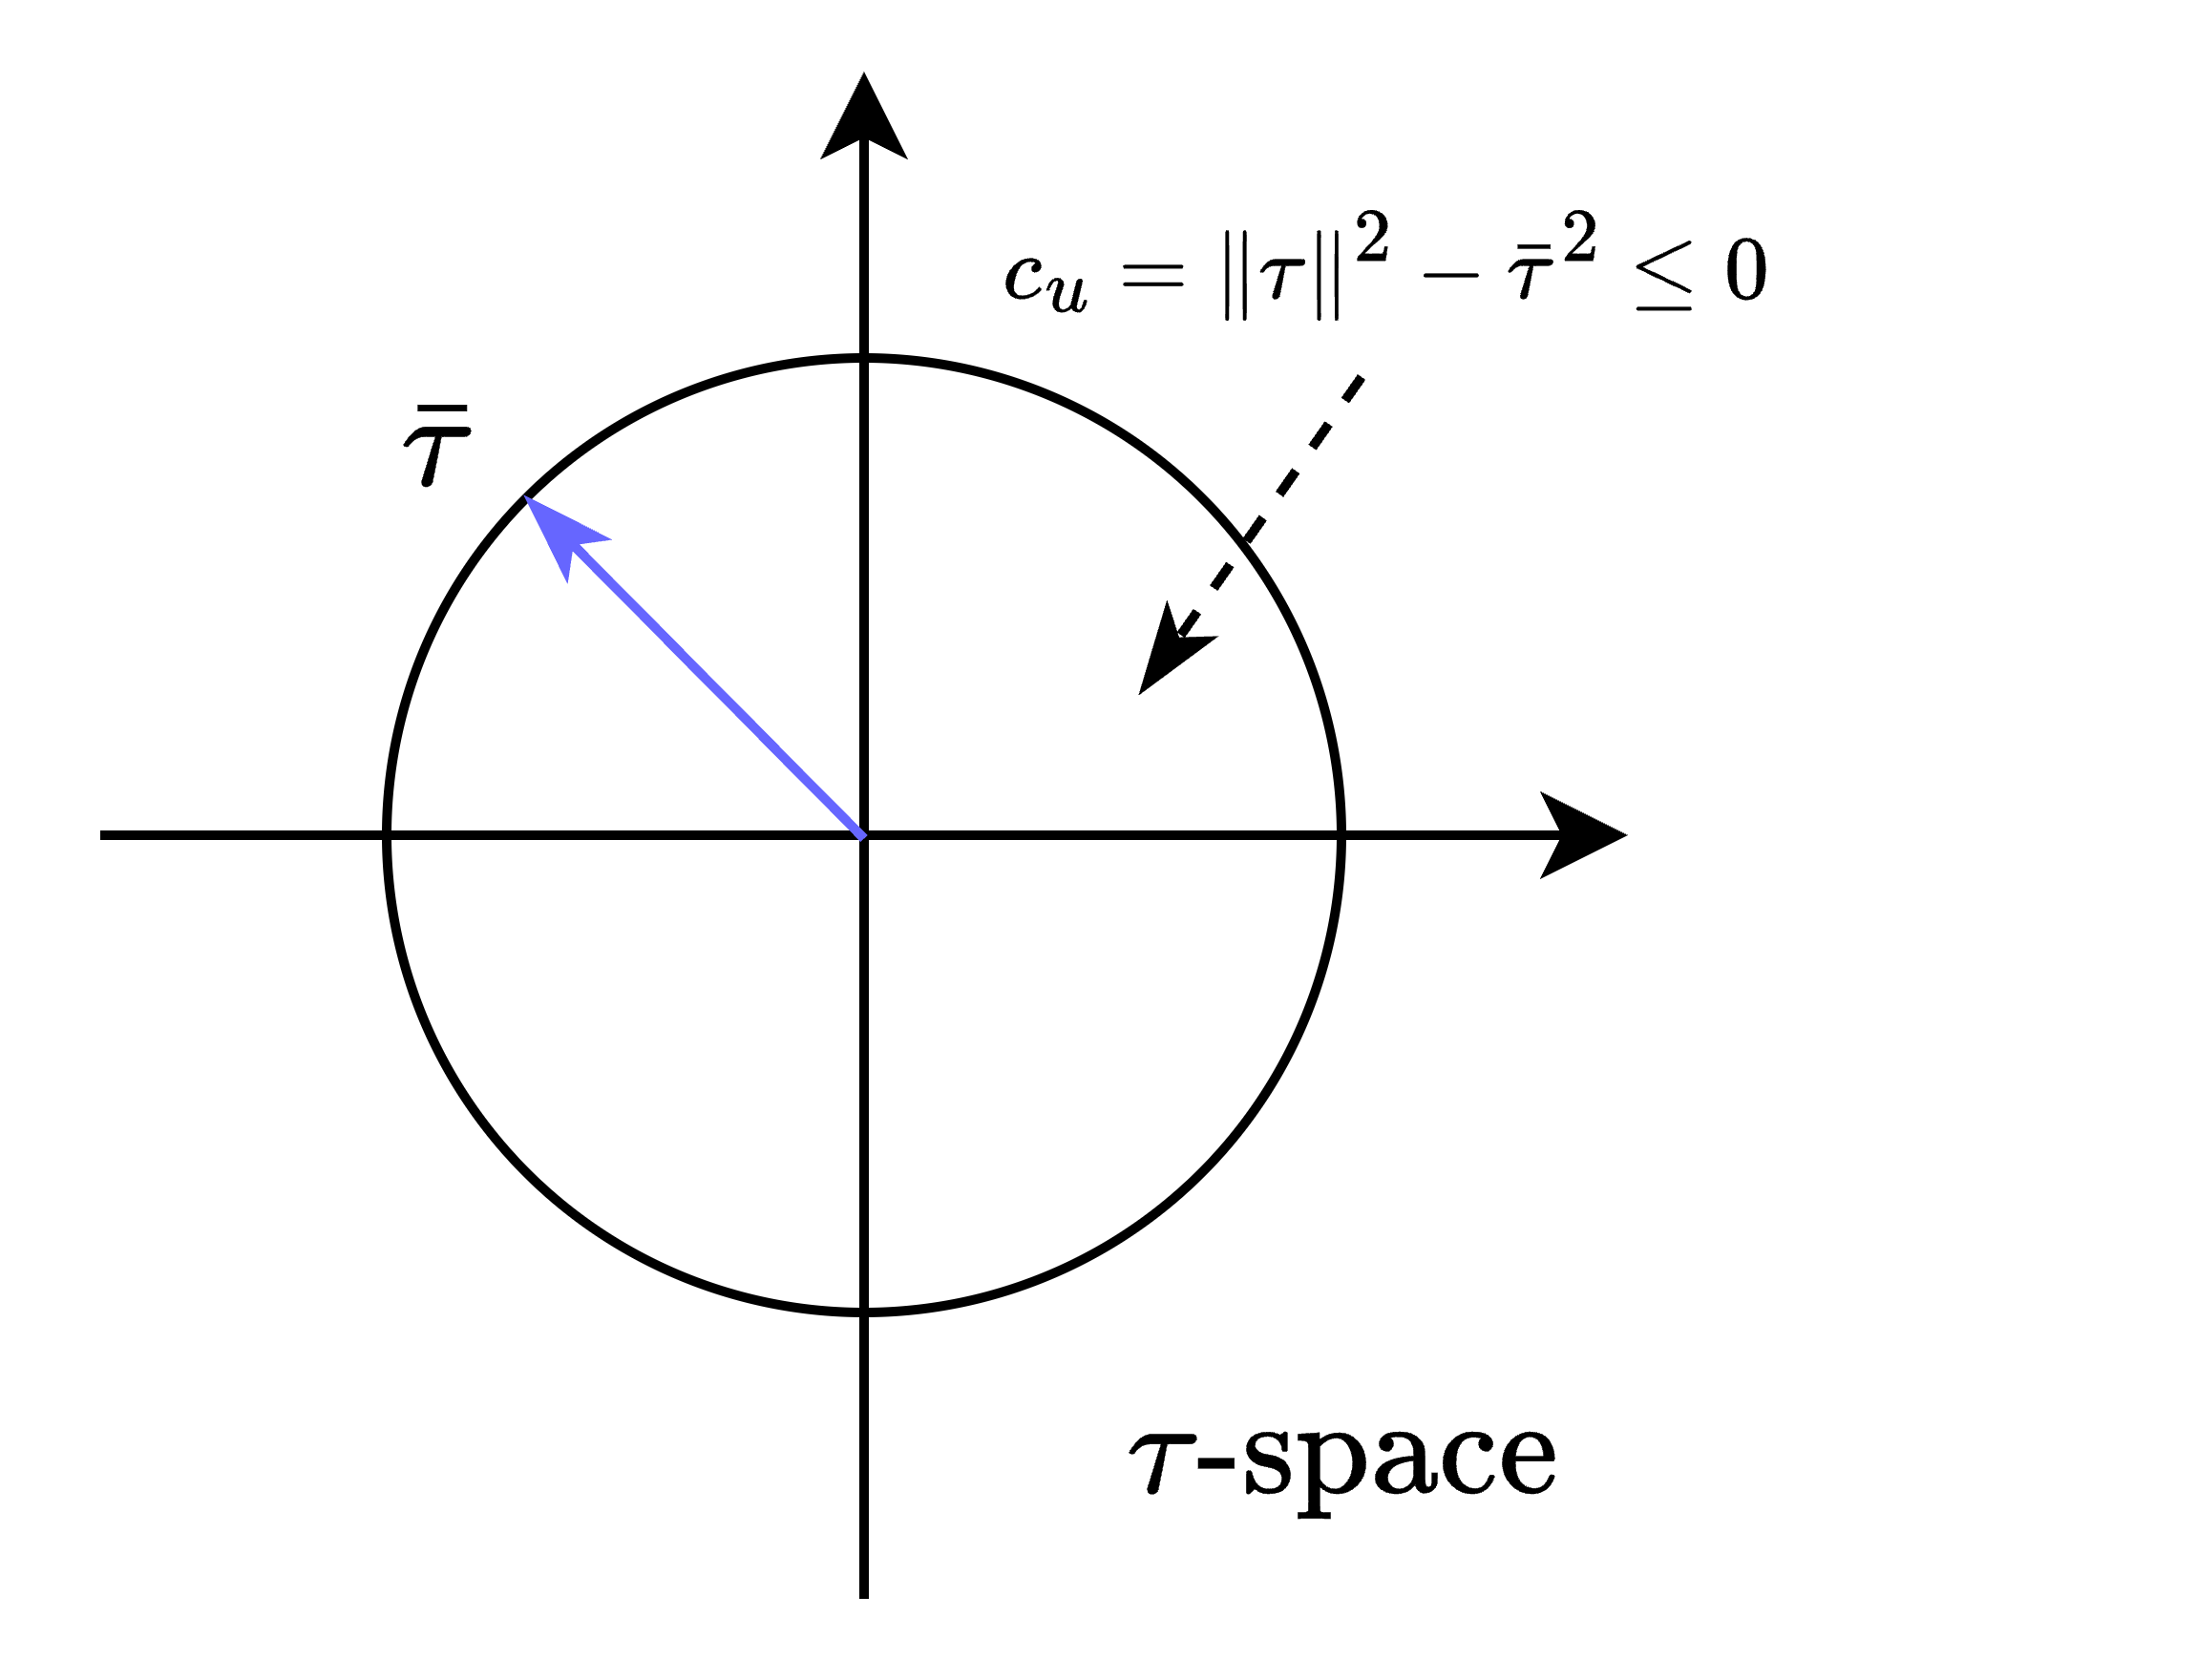
\includegraphics[width=0.5\linewidth]{imgs/cstr_input_norm.drawio.png}
    \caption{Input norm constraints.}
    \label{chap4:fig:cstr:u_norm}
\end{figure*}

Consider the control input $\tau$ as the torque of each actuator corresponding to its generalized coordinate. 
Since torque is typically linearly proportional to current, actuators that share a common power source are often subject to total current limitations. 
This can be captured by the following inequality constraint: 
\begin{equation}
    c_{u}=\Vert\tau\Vert^2 -\bar\tau^2  \le 0
    \label{chap4:eq:cstr:input_norm}
\end{equation}
with $\bar\tau\in\R_{>0}$ denoting the maximum allowable control input magnitude as shown in Fig.~\ref{chap4:fig:cstr:u_norm}. 
This input norm constraint is also commonly applied in current and torque control problems for electric motors \cite{RN90}.
% The corresponding Lagrangian multipier is $\lambda_{u_b}$. 
The gradients of $c_{u}$ with respect to $\hat\theta$ are given by
\begin{equation}
    {\partial \mathbf \mathbf c_{u} \over \partial \hat\theta}
    = -\sum_{i=1}^n 2\tau_{(i)} 
    \bigg(
        \text{row}_i
        \bigg(
            -{\partial \hat\Phi\over\partial\hat\theta}
        \bigg)
    \bigg)^T  
    = \tau^T (I_{l_{k+1}}\otimes \hat\phi_k^T)
    \in \R^{\Xi}.
    \label{chap4:eq:cstr:input_norm_grad}
\end{equation}
It should be noted that constraints \eqref{chap4:eq:cstr:input_bound} and \eqref{chap4:eq:cstr:input_norm} cannot be imposed simultaneously, as their gradients \eqref{chap4:eq:cstr:input_bound_grad} and \eqref{chap4:eq:cstr:input_norm_grad} are linearly dependent, violating the LICQ condition (see Definition \ref{chap2:def:LICQ}).

%%%%%%%%%%%%%%%%%%%%%%%%%%%%%%%%
\section{Stability Analysis} 
%%%%%%%%%%%%%%%%%%%%%%%%%%%%%%%%

Before conducting the stability analysis, let $\tilde\theta\triangleq [\tilde\theta_i]_{i\in[0,\cdots,k]}$, where $\tilde\theta_i\triangleq\hat\theta_i-\theta^*_i$ represents the weight estimation error. 
The following Lemmas are introduced for the stability analysis. % of the last layer of the DNN.
\begin{lemma}
    If Assumptions \ref{chap4:assum:assum1} and \ref{chap4:assum:assum2} are satisfied, the angle between $\partial c_j/\partial \hat\theta_k$ and $\hat\theta_k$ is positive when $c_j$ is active set, \ie $(\partial c_j/\partial \hat\theta_k)^T\hat\theta_k>0$.
    \label{chap4:lem:lem1}
\end{lemma}

\begin{figure}[!t]
   \centering
   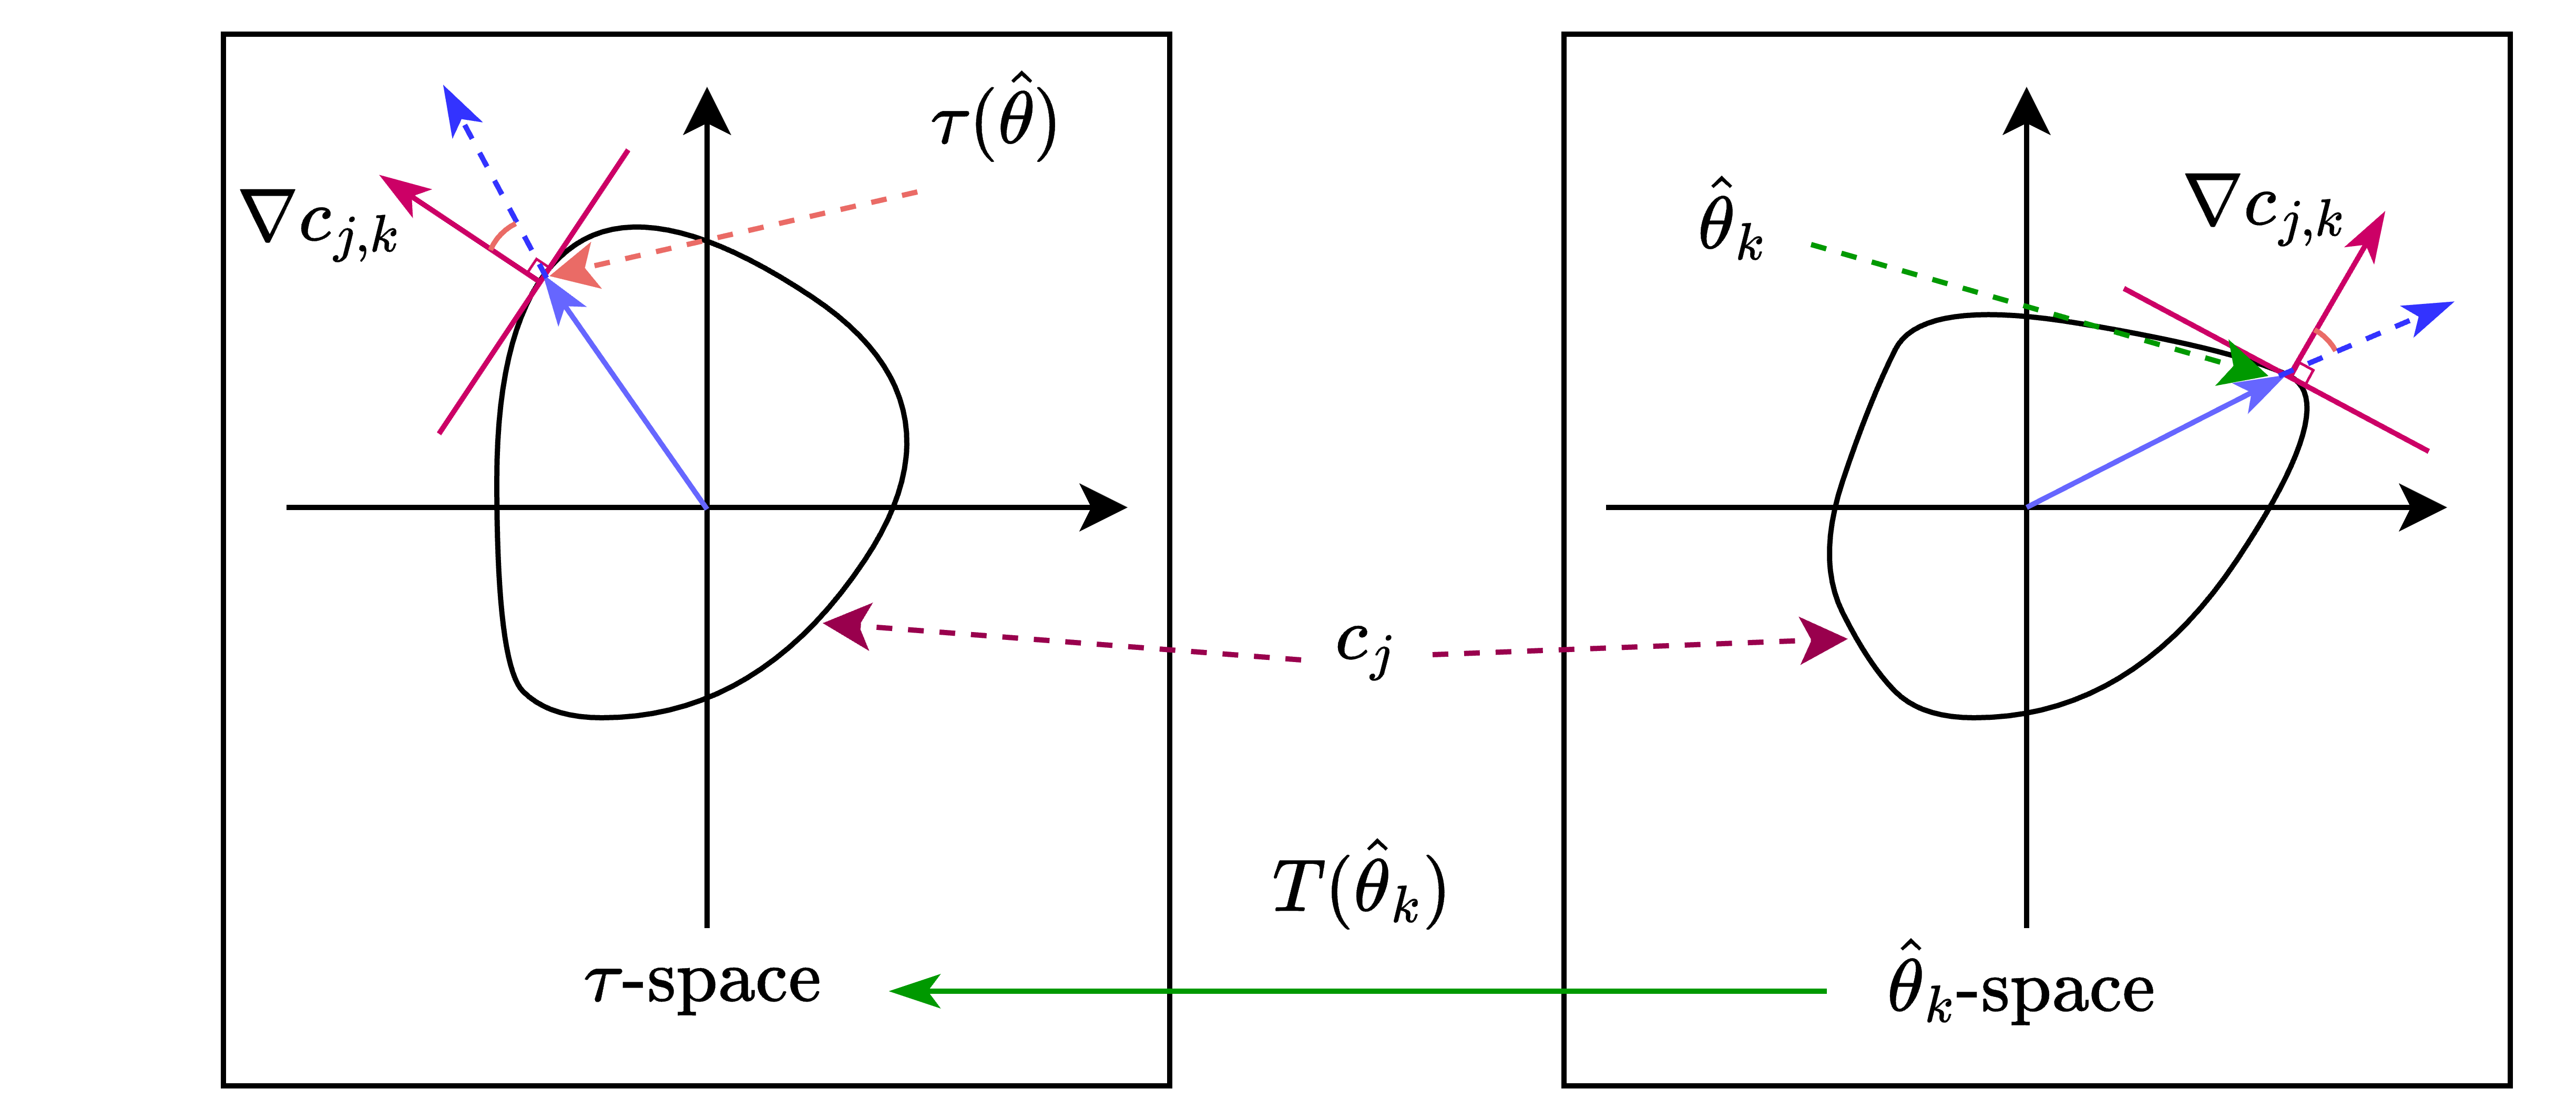
\includegraphics[width=.9\linewidth]{imgs/spaces.drawio.png}
   \caption{Convexity of input constraints.}
   \label{chap4:fig:spaces}
\end{figure}

\begin{proof}

Since $\tau = -\hat\Phi$, using Proposition \ref{chap2:prop:kron}, a linear map $T(\cdot):\hat\theta_k\to\tau$ can be derived as follows: 
\begin{equation}
    \begin{aligned}
    \tau = &-\hat\Phi = -\text{vec}(\hat\Phi)     
    = -\text{vec}(\hat V_k \hat\phi_k) 
    \\
    = & -(I_{l_{k+1}}\otimes \hat\phi_k^T)\text{vec}(\hat V_k)
    =-(I_{l_{k+1}}\otimes \hat\phi_k^T)\hat\theta_k = T(\hat\phi_k) \hat\theta_k
    .
    \end{aligned}
    \label{chap4:eq:linear map}
\end{equation}
Therefore, since the linear map is affine map, the convexity of the input constraints in $\tau$-space (assumed in Assumption \ref{chap4:assum:assum1}) holds in $\hat\theta_k$-space as well as discussed in Section \ref{chap2:sec:convex_preserve}, implying that $(\partial c_j/\partial \hat\theta_k)^T\hat\theta_k>0$ (see Lemma \ref{chap2:lem:conv_ang}).
The preservation of convexity is illustrated in Fig.~\ref{chap4:fig:spaces}.

\end{proof}

\begin{lemma} 
    If $c_j(\hat\theta),\ \forall j\in\mathcal I \setminus \{\theta_i\}_{i\in[0,\cdots,k]}$ satisfies Assumption \ref{chap4:assum:assum1}, then $\Vert\partial c_j/\partial\hat\theta_i\Vert \allowbreak $, for all $i\in[k-1,\cdots, 0]$, is bounded, provided the norms of $\hat\theta_i$, for all $i\in[k,\cdots, i+1]$, remain bounded.
    \label{chap4:lem:lem2}
\end{lemma}

\begin{proof}

The derivative of $c_j,\ \forall j\in\mathcal I \setminus \{\theta_i\}_{i\in[0,\cdots,k]}$, with respect to $\hat\theta_i$ is represented as
\begin{equation}
    {\partial c_j\over\partial \hat\theta_i} = {\partial c_j\over\partial \tau} {\partial \tau\over\partial \hat\Phi} {\partial \hat\Phi\over\partial \hat\theta_i}
\end{equation}
where $\partial \tau/\partial \hat\Phi=-I_n$, which is bounded. 
From the linear mapping in \eqref{chap4:eq:linear map}, $\tau$ is bounded as long as $\hat\theta_k$ is bounded (by the condition of the lemma), and $\Vert\phi_k(\cdot)\Vert$ is bounded due to the properties of the activation functions. 
By Assumption \ref{chap4:assum:assum1}, the function $c_j$ is convex. 
The convex function has a bounded derivative with respect to $\tau$, since $\tau$ is a bounded variable (\ie $\partial c_j/\partial\tau$ is bounded). 
Furthermore, $\partial \hat\Phi/\partial \hat\theta_i$ is bounded, provided that the norms of $\hat\theta_i,\ \forall i \in[k,\cdots,i+1]$, are bounded. 
This can be verified using the definition of $\partial \hat\Phi/\partial\hat\theta_i$ given in \eqref{chap2:eq:DNNgrad}.
Consequently, $\Vert\partial c_j/\partial \hat\theta_i\Vert,\ \forall j\in\mathcal I \setminus \{\theta_i\}_{i\in[0,\cdots,k]}$, is bounded, when $\hat\theta_i,\ \forall i\in [k,\cdots,i+1]$ are bounded.

\end{proof}

The following theorem shows that $\hat\theta$ and $\xi$ are bounded.

\begin{theorem}
    For the dynamical system in \eqref{chap4:eq:sys1}, the neuro-adaptive controller \eqref{chap4:eq:approx_control} and weight adaptation laws \eqref{chap4:eq:adap} ensure the boundedness of the augmented error $\xi$ and the weight estimate $\hat \theta$. This holds with the weight norm constraint \eqref{chap4:eq:cstr:weight} and input constraints satisfying Assumption \ref{chap4:assum:assum2} and \ref{chap4:assum:assum2}, provided that the control gains ${k_q}$ and ${k_z}$ satisfy \eqref{chap4:eq:stable_cond}.
\end{theorem}

\begin{proof}

The boundednesses of $\hat\theta$, $\xi$, and $\eta$ are analyzed recursively from the last $k\textsuperscript{th}$ layer to the first layer of $\hat\Phi$. 
The step-by-step analysis is described as follows.

\subsubsection{
    Step 1: Boundedness of $\hat\theta_k,\eta_k$, and $\xi$
}

The boundedness of $\xi$ follows from \eqref{chap4:eq:xi_dyna}, using Theorem \ref{chap2:thm:BIBO}, since $A_\xi$ is a stable matrix and the term $B_\xi (\Phi^*-h(\hat\Phi)+\epsilon)$ is bounded due to $\Vert B_\xi\Vert_F$, $\Vert V_k^*\Vert_F$, $\Vert \phi(\cdot)\Vert$, $\Vert h(\cdot)\Vert$, and $\Vert\epsilon\Vert <\infty$.

Assume that all constraints are in active set $\mathcal A$ without loss of generality. 
The dynamics of $\eta_k$ and $\hat\theta_k$ can be decomposed from \eqref{chap4:eq:adap_th} and \eqref{chap4:eq:eta_dyna} as 
\begin{equation}
    \begin{aligned}
        \dot\eta_k =
        & 
        A_\xi \eta_k -B_\xi {\partial h\over\partial\tau}{\partial \hat\Phi\over \partial \hat\theta_k}
        =
        A_\xi \eta_k -B_\xi {\partial h\over\partial\tau}(I_{l_{k+1}}\otimes \hat\phi_k^T)\\
        \dot{\hat\theta}_k =
        & -\alpha 
        \bigg[
            \eta_k^TW\xi+
            \sum_{j\in\mathcal{A}}
            \lambda_j{\partial c_j\over\partial \hat\theta_k}
        \bigg]
    \end{aligned} 
\end{equation}
According to Theorem \ref{chap2:thm:BIBO}, $\Vert \eta_k\Vert_F$ is bounded, since $A_\xi$ is a stable matrix and the term $-B_\xi(\partial h/\partial \tau)(I_{l_{k+1}}\otimes\hat\phi_k^T)$ is also bounded.

Let $\mathcal{V}: \R^{2n} \times \R^{\Xi} \to \R_{>0}$ denote the Lyapunov function:
\begin{equation}
    \mathcal{V} = \frac{1}{2} \xi^T P \xi + \frac{1}{2 \alpha} \hat{\theta}_k^T \hat{\theta}_k,
\end{equation}
with the Lyapunov equation $A_\xi^T P + P A_\xi = -Q$, where $A_\xi < 0$, $P = P^T > 0$, and $Q > 0$.
Taking the time derivative of $\mathcal{V}$ yields:
\begin{equation}
    \dot{\mathcal{V}} 
    = -\frac{1}{2} \xi^T Q \xi + \xi^T P B (V_k^{*T} \phi_k^* - h(\tau) + \epsilon)
    - \hat{\theta}_k^T \left( \eta_k W \xi + \sum_{j \in \mathcal{A}} \lambda_j \frac{\partial c_j}{\partial \hat{\theta}_k} \right)
    .
\end{equation}
By applying the boundedness of $\Delta \triangleq P B (V_k^{*T} \phi_k^* - h(\tau) + \epsilon)$ and $M \triangleq \eta_k W$, where $\Vert \Delta \Vert \leq \bar{\Delta} < \infty$ and $\Vert M \Vert_F \leq \bar{M} < \infty$, this simplifies to:
\begin{equation}
    \dot{\mathcal{V}} 
    \leq \left( -\frac{\lambda_{\text{min}}(Q)}{2} + \frac{\bar{M}}{2} \right) \Vert \xi \Vert^2 + \bar{\Delta} \Vert \xi \Vert 
        + \frac{\bar{M}}{2} \Vert \hat{\theta}_k \Vert^2 - \sum_{j \in \mathcal{A}} \lambda_j \hat{\theta}_k^T \frac{\partial c_j}{\partial \hat{\theta}_k}
        .
    \label{chap4:eq:V1_dot}
\end{equation}
Representing the term $\partial c_{\theta_k}/\partial \hat\theta_k$ in the last inequality as $\partial c_{\theta_k}/\partial \hat\theta_k=2\hat\theta_k$ and using the result provided in \eqref{chap4:eq:cstr:weight_grad}, $\dot {\mathcal V}$ can be rewritten as
\begin{equation}
    \begin{aligned}
        \dot {\mathcal V} \le&
        (\cdot) + 
        \bigg(
            -2\lambda _{\theta_k}+{\bar M}/{2}
        \bigg)
        \Vert\hat\theta_k\Vert^2 
        - \underbrace{
        \sum_{j\in\mathcal{A}\setminus \{\theta_i\}_{i\in[0,\cdots,k]}}\lambda_j\hat\theta_k^T{\partial c_j\over\partial \hat\theta_k}
        }_{>0, \text{\;by Lemma} \ref{chap4:lem:lem1} \text{\;and\;} \text{Assumption} \ref{chap4:assum:assum2}}	
        \\
        \le&
        \bigg(
            -{\lambda_\text{min}(Q)}/{2}+{\bar M}/{2}
        \bigg)
        \Vert\xi\Vert^2
        +\bar \Delta \Vert \xi\Vert 
        + 
        \bigg(
            -2\lambda _{\theta_k}+{\bar M}/{2}
        \bigg)
        \Vert\hat\theta_k\Vert^2 
    \end{aligned}
    \label{chap4:eq:V2_dot}
\end{equation}
Define $P=I_2$, leading to $Q = -A_{\xi}^T - A_{\xi}$. 
Consequently, the minimum eigenvalues ${\lambda_{\text{min}}(Q)}$ is determined by $2\min({k_q},{k_z})$, as follows from the structure of the matrix $A_{\xi}$. 
From \eqref{chap4:eq:V2_dot}, if the control gains ${k_q}$ and ${k_z}$ are chosen sufficiently large to satisfy the condition:
\begin{equation}
    % -\lambda_\text{min}(Q)/2+M/2<0
    \min({k_q},{k_z})>\bar M/2
    \label{chap4:eq:stable_cond}
\end{equation}
and if the Lagrange multiplier $\lambda_{\theta_k}$ for the weight norm constraint of the $k\textsuperscript{th}$ layer is increased sufficiently, such that
\begin{equation}
    -2\lambda_{\theta_k} +{\bar M/ 2}<0,  
\end{equation}
(as dictated by \eqref{chap4:eq:adap_L} when the corresponding constraint is violated, \ie $c_{\theta_k}=\Vert \hat\theta_k\Vert^2 -\bar\theta_k^2 > 0$), then both $\xi$ and $\hat\theta_k$ will remain bounded within the compact sets $\Theta_\xi$ and $\Theta_{\hat\theta_k}$, defined as
\begin{equation}
    \Theta_\xi = 
    \bigg\{ \xi \ \bigg\vert\ \Vert\xi\Vert \le  
    {2\bar \Delta\over \lambda _\text{min}(Q)-\bar M} 
    \bigg\}
\end{equation}
and
\begin{equation}
    \Theta_{\hat\theta_k} = 
    \{
    \hat\theta_k 
    \ 
    \vert
    \ 
    \Vert
    \hat\theta_k\Vert \le  
    \bar\theta_k
    \}
    .
\end{equation}
The increase of the Lagrange multiplier $\lambda_{\theta_k}$ will halt once $\hat \theta_k$ reaches the compact set $\Theta_{\hat\theta_k}$. 
Thus, the Lagrange multiplier $\lambda_{\theta_k}$ is bounded.

The boundedness of the Lagrange multipliers $\lambda_j,\ \forall j\in\mathcal A\setminus\{\theta_i\}_{i\in[0,\cdots,k]}$, can be accessed by considering the convexity of the constraints in $\hat\theta_k$-space.
The boundedness of the remaining Lagrange multipliers associated with the weight norm constraints, $\lambda_{\theta_r},\ \forall r\in[0,\cdots,k-1]$, will be examined in Step $i$. 
Based on Assumption \ref{chap4:assum:assum1} and Lemma \ref{chap4:lem:lem1}, the equality constraints $c_j \le 0, \ \forall j\in\mathcal A\setminus \{\theta_i\}_{i\in[0,\cdots,k]}$, for convex sets $\Theta_{c_j}$ in $\hat\theta_k$-space.
Let $\Theta_c\triangleq \cap_{j\in\mathcal A\setminus \{\theta_i\}_{i\in[0,\cdots ,k]}} \Theta_{c_j}$ represent the intersection of these convex sets, which also contains the origin.
If $\lambda_j$ increases sufficiently such that $\dot{\mathcal V} \approx -\sum_{j\in\mathcal A\setminus \{\theta_i\}_{i\in[0,\cdots,k]}}\lambda_j\hat\theta_k^T(\partial c_j/\partial \hat\theta_k)<0$, then ${\mathcal V}$, and consequently $\Vert\hat\theta_k\Vert$, will decrease until $\hat\theta_k$ reaches $\Theta_\xi\cap\Theta_{\hat\theta_k}\cap\Theta_c$. Once $\hat\theta_k$ hits the boundary of $\Theta_c$, the Lagrange multipliers will cease to increase, thus ensuring their boundedness.

\subsubsection{Step i: Boundedness of $\hat\theta_i$ and $\eta_i, \ i\in[k-1,\cdots,0]$}

The boundedness of the Frobenius norm of the gradient $\partial\hat\Phi/\partial \hat\theta_i$ can be obtained from its definition in \eqref{chap2:eq:DNNgrad}. 
This relies on the fact that the boundedness of $\Vert\hat\theta_i\Vert,\ \forall i\in[k,\cdots,i+1]$, was already shown in the previous step (\ie Step 1 to Step $i+1$) and the activation functions $\hat\phi_i$ and their derivative $\hat\phi_i'$ are bounded.

The dynamics of $\eta_i$ and $\hat\theta_i$ for all $i\in [k-1,\cdots,0]$ are represented as
\begin{equation}
    \dot\eta_i = 
    A_\xi\eta_i -B_\xi {\partial h\over\partial\tau}
    {\partial \hat\Phi\over \partial \hat\theta_i}
\end{equation}
and
\begin{equation}
    \dot{\hat\theta}_i 
    =
    -\alpha 
    \bigg[
        \eta_i^TW\xi+2\lambda_{\theta_i} \hat\theta_i
        +
        \sum_{j\in\mathcal{A}\setminus \{\theta_i\}_{i\in[0,\cdots,k]}}\lambda_j{\partial c_j\over\partial \hat\theta_i}
    \bigg]
    .
\end{equation}
According to Theorem \ref{chap2:thm:BIBO}, $\Vert\eta_i\Vert_F$ is bounded because $A_\xi$ is a stable matrix and the terms $\Vert B_\xi\Vert, \Vert(\partial h/\partial \tau)\Vert_F$, and $\Vert\partial \hat\Phi/\partial\hat\theta_i\Vert_F$ are bounded.
When $\lambda_{\theta_i}$ is generated due to a violation of the weight norm constraint, $\hat\theta_i$ remains bounded because the term $-2\alpha\lambda_{\theta_i}$ is stable, and the residual terms $\Vert\eta_iW\xi\Vert$, $\lambda_j$, and $\Vert(\partial c_j/\partial \hat\theta_i)\Vert_F$ for all $j\in\mathcal{A}\setminus \{\theta_i\}_{i\in[0,\cdots,k]}$ are bounded, as demonstrated in Step 1 and by Lemma \ref{chap4:lem:lem2}.
The boundedness of each $\lambda_{\theta_i}$ also can be obtained, assuming that $\lambda_{\theta_i}$ is sufficiently increased regulating $\Vert\theta_i\Vert$ into the origin until $c_{\theta_i}$ is satisfied.

Therefore, starting from the boundedness of $\xi$, $\hat\theta_k$, and $\eta_k$ in the $k\textsuperscript{th}$ layer, the boundednesses of $\hat\theta_i$ and $\eta_i$ for the remaining layers $i\in[0,\cdots,k-1]$ can be established recursively, down to the input layer ($i=0$). 
Thus, $\hat\theta$, $\xi$, and $\eta$ are bounded because $\hat\theta_i,\eta_i,\ \forall i\in[0,\cdots,k]$ and $\xi$ are bounded. Furthermore, since the estimated weight vector $\hat\theta$ is bounded, the weight estimation error $\tilde\theta$ is also bounded, as $\theta^*$ is bounded according to the universal approximation theorem.

\end{proof}

%%%%%%%%%%%%%%%%%%%%%%%%%%%%%%%%
\section{Simulation Validation} 
%%%%%%%%%%%%%%%%%%%%%%%%%%%%%%%%

\subsection{Setup}

The proposed CoNAC was validated using a two-link manipulator model, as depicted in Fig.~\ref{chap4:fig:plant}, adapted from \cite{RN33}. 
The parameters $q_p,{q_d}_p,\tau_p,m_p,l_p,{l_c}_p,b_p$, and ${f_c}_p$ denote the joint angle, desired joint angle, torque, mass, length, center of mass, viscous coefficient, and friction coefficient, respectively, for link $p\in[1,2]$.
%This model contains terms of gravity and friction in its mechanical system.
%These terms make system functions in \eqref{eq. system dynamics 1} nonlinear.
%and can be considered as the disturbance of the system.
The values of the system model parameters are provided in Table~\ref{chap4:table:plant_param}. The desired trajectory for ${q}=[q_1,q_2]^T$ was defined as
\begin{equation}
    {q_d}(t) = 
    \begin{bmatrix}
        {q_d}_1\\{q_d}_2
    \end{bmatrix}
    =
    \begin{bmatrix}
        +\cos(0.49\pi t) + 1 \\
        -\cos(0.49\pi t) - 1 
    \end{bmatrix}.
\end{equation}
%\color{red}
%Considering the power limitation of the power source for the actuators [], 
The control input saturation function was defined as $h(\tau)\triangleq \tau/\Vert\tau\Vert \cdot \text{SSF}_L^U(\Vert\tau\Vert)$, where smooth saturation function (SSF) was adopted from \cite{RN72} and is given by
\begin{equation}
    \text{SSF}_L^U(\Vert\tau\Vert) = {\Vert\tau\Vert\over (1+(\Vert\tau\Vert/\bar\tau)^p)^{1/p}}.
    \label{chap4:eq:sat_h}
\end{equation}
with $p$ being the smoothing factor. 
The effect of $p$ and the boundedness of $\Vert\partial h/\partial \tau\Vert_F$ is shown in Fig.~\ref{fig: h func}.
The parameters of the control input saturation function were selected as $p=100$ and $\bar\tau=50$. 

In addition to this physically imposed control input saturation, the input norm constraint \eqref{chap4:eq:cstr:input_norm} was imposed to ensure that the control input $\tau$ stays within the unsaturation region of $h(\tau)$ and to prevent inefficient use of the input. 
With a sufficiently large value for $p$, the input norm constraint essentially matches the control input saturation function. 
Note that among the selected controllers given below, only the proposed CoNAC can rigorously handle this input norm constraint.

% **********************************************************
% SYSTEM FIGURE AND TABLE
\begin{figure}[!t]
    \centering
    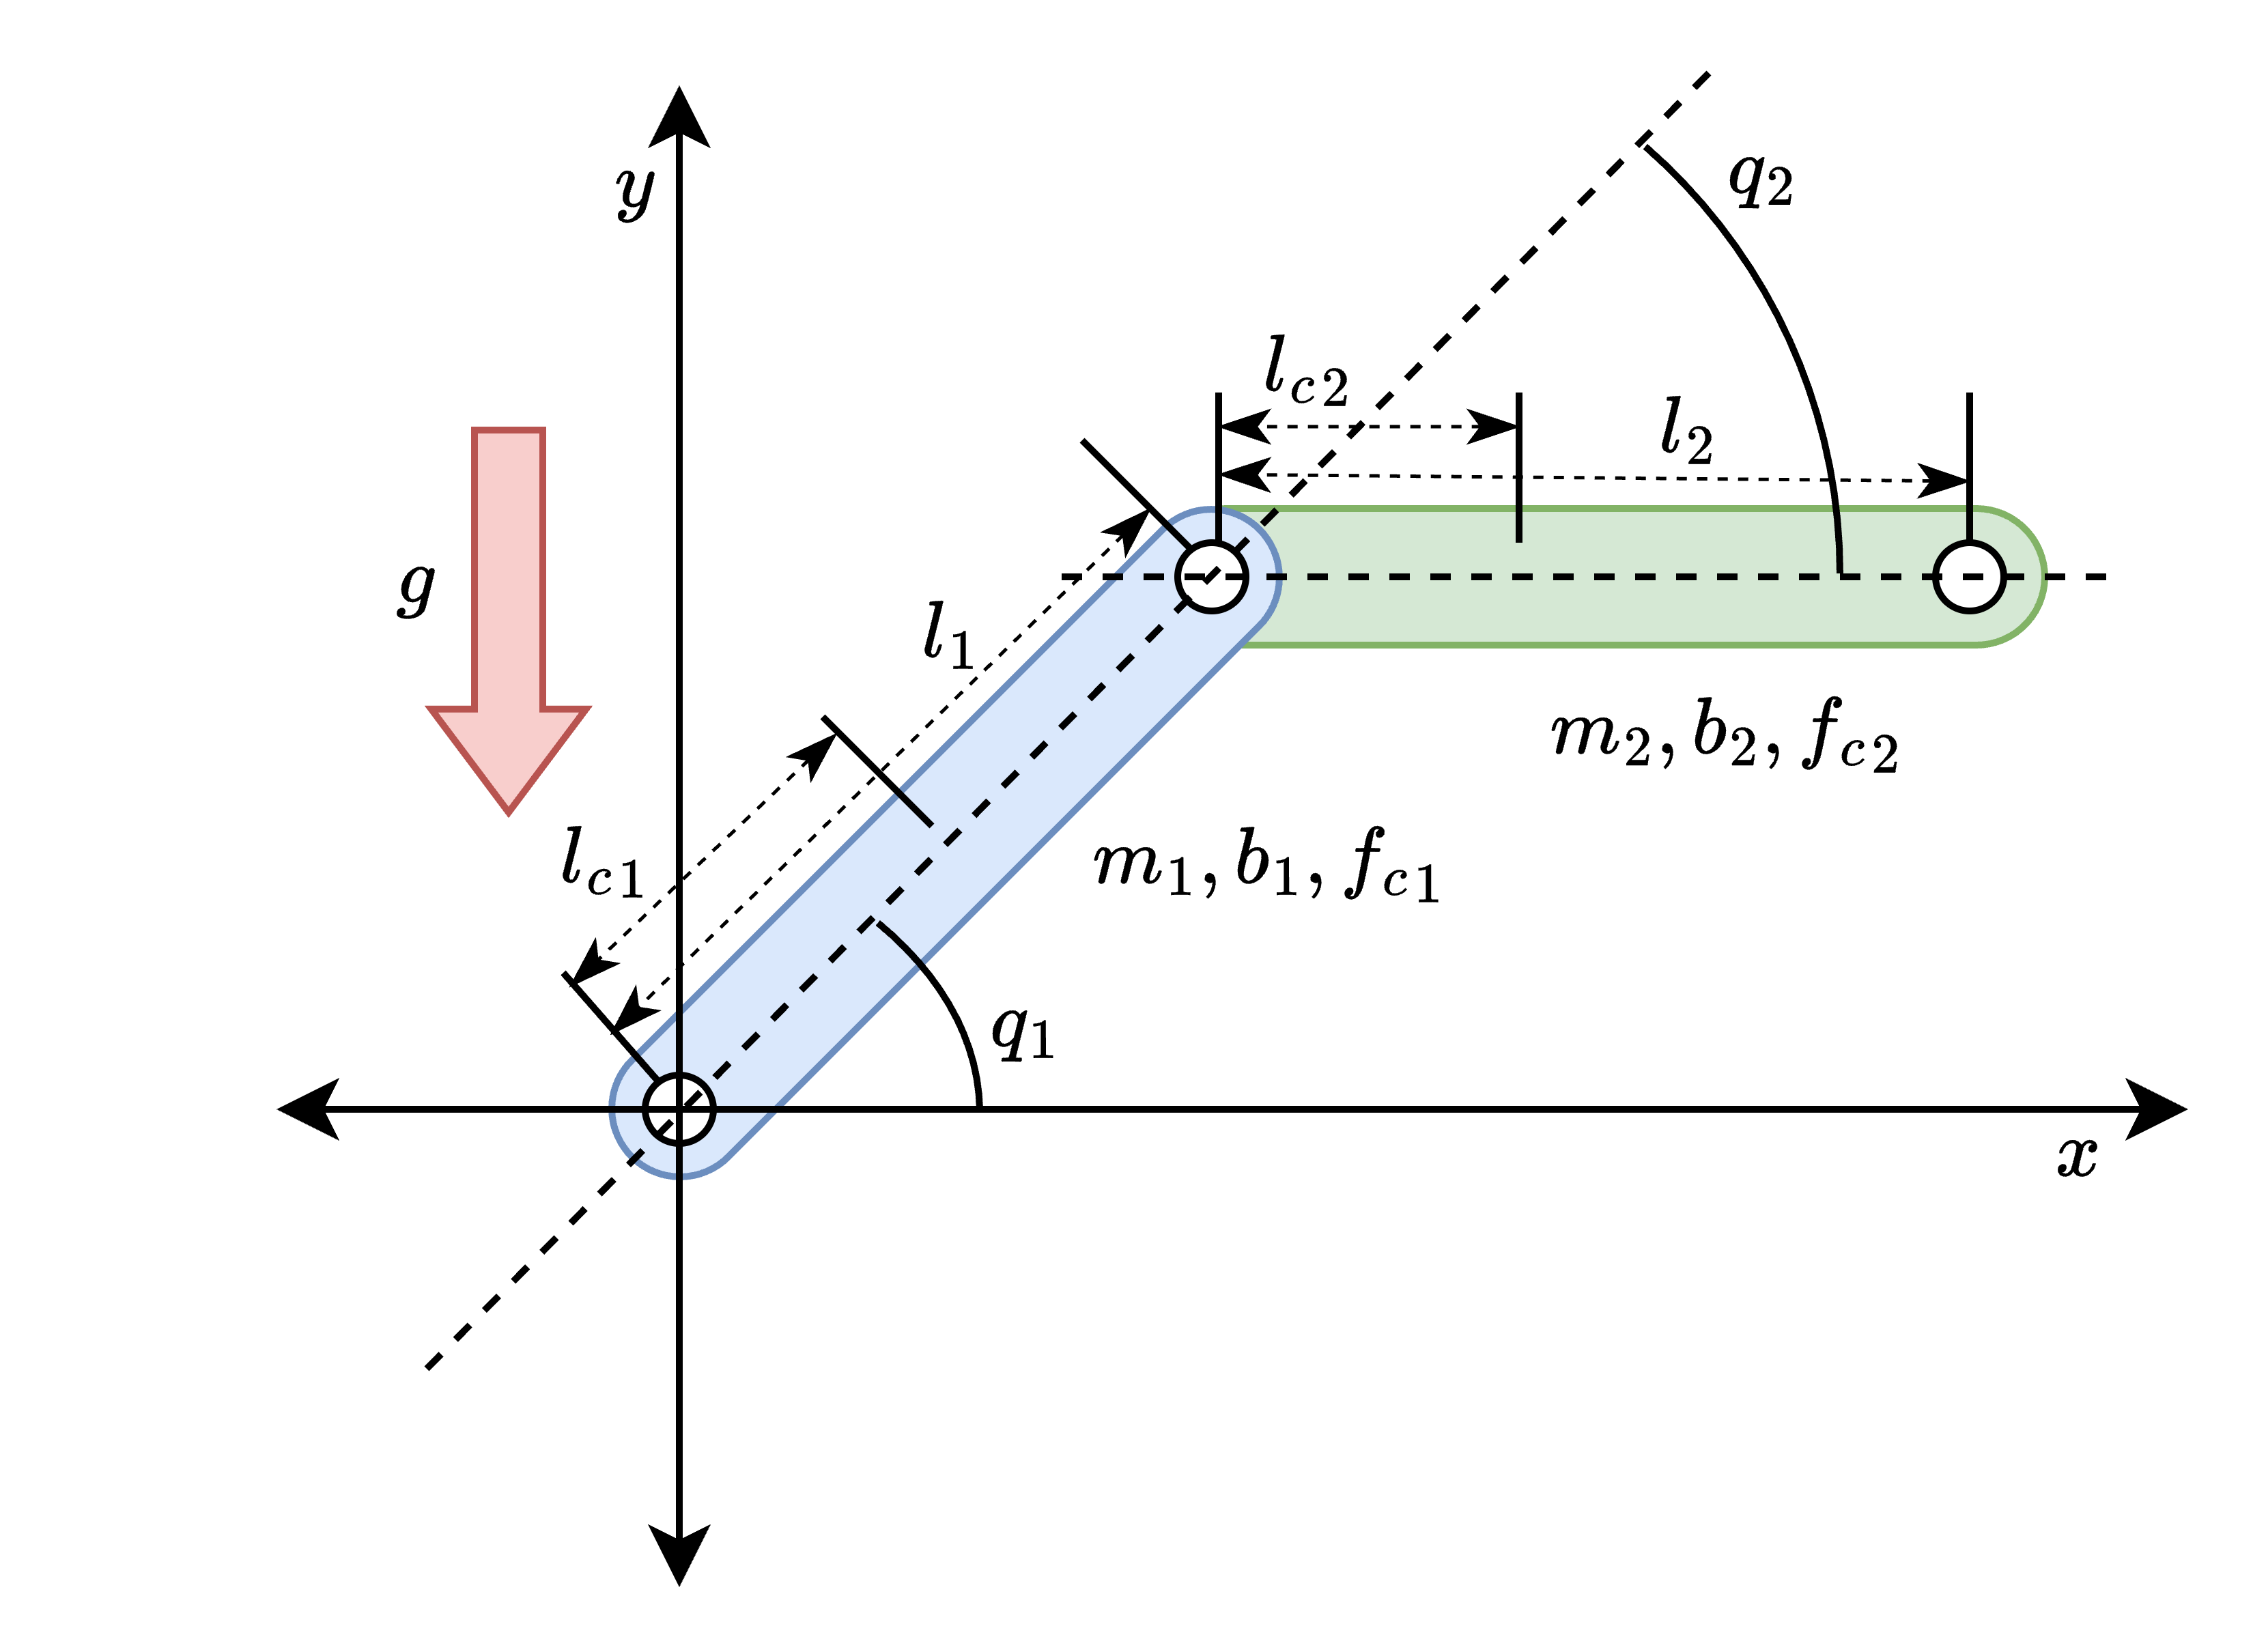
\includegraphics[width=0.7\linewidth]{imgs/RobotModel.drawio.png}
    \caption{Two-link manipulator model.}
    \label{chap4:fig:plant}
\end{figure}

\begin{table}[!t]
    \renewcommand{\arraystretch}{1.3}
    \caption{System model parameters.}
    \centering
    \begin{tabular}{|c||c|c|c|c|}
    \hline
    Symbol & \textbf{Description} & \textbf{Link 1} & \textbf{Link 2} \\
    \hline 
    $m_1, m_2$ & Mass of link    & 23.902 (kg) & 3.88 (kg) \\
    \hline
    $l_1, l_2$  & Length of link   & 0.45 (m) & 0.45 (m) \\
    \hline
    $l_{c1}, l_{c2}$ & COM of link  & 0.091 (m) & 0.048 (m) \\
    \hline
    $b_1, b_2$   & Viscous coefficient  &  2.288 (Nms) & 0.172 (Nms) \\
    \hline
    $f_{c1}, f_{c2}$  & Friction coefficient &  7.17 (Nm) & 1.734 (Nm) \\
    \hline
    \end{tabular}
    \label{chap4:table:plant_param}
\end{table}

\begin{figure}[!t]
    \centering
    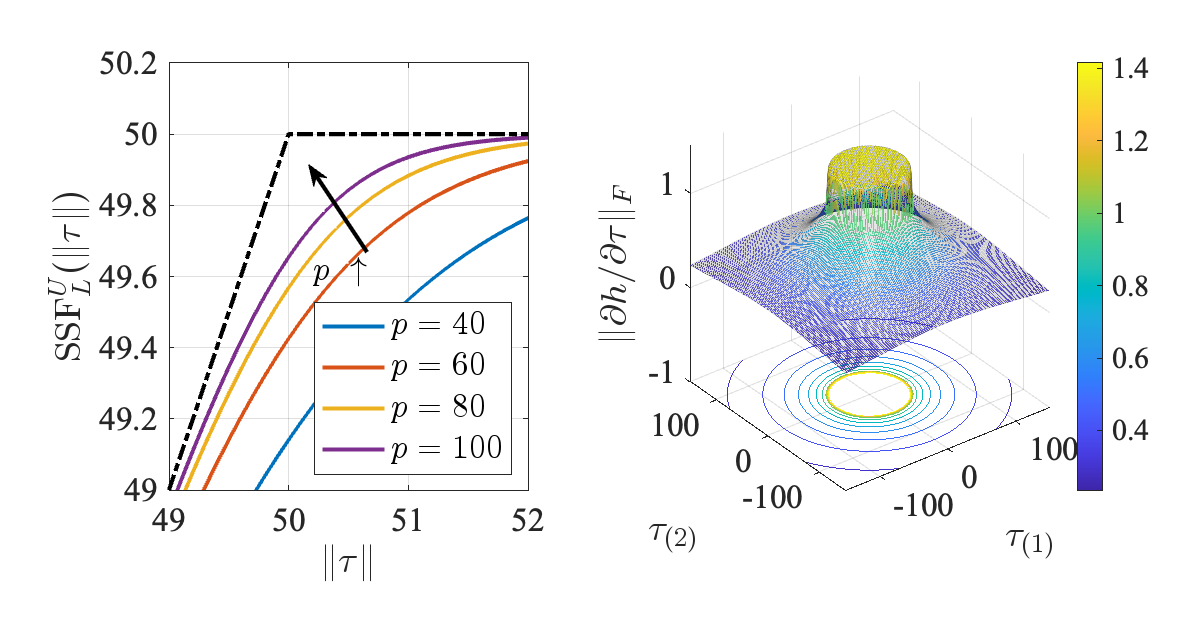
\includegraphics[width=0.85\linewidth]{imgs/Chap4/fig13.eps}
    \caption{Effect of parameter $p$ in the control input saturation function $h$ and boundedness of $\Vert\partial h/\partial \tau\Vert_F$.}
    \label{fig: h func}
\end{figure}

% SYSTEM FIGURE AND TABLE
% **********************************************************
Four controllers were examined for a comparative study. 
The first was the Backstepping Controller (BSC), used as the baseline. 
The second was the DNN-based Backstepping Controller (DNN-BSC), an existing neuro-adaptive control method where a DNN was employed to learn and compensate for the lumped system uncertainty function $f$ in the BSC. 
While this method addressed the weight norm constraint via a projection operator, it did not account for either the input norm or input bound constraints. 
The third was DNN-BSC augmented with an auxiliary system presented in \cite{RN95,RN46,RN60} (DNN-BSC-A), which handled the (linear) input saturation constraint but not the nonlinear input norm constraint. 
As a result, an approximation of the input norm constraint was used as an input bound constraint. 
Lastly, the proposed controller, CoNAC, rigorously considered system uncertainties, the weight norm constraint, and input constraints within a constrained optimization framework. The properties of these four controllers are summarized in Table \ref{chap4:table:ctrl}.

\begin{table}[!t]
    \renewcommand{\arraystretch}{1.3}
    \caption{Properties of the controllers used in simulation.}
    \label{chap4:table:ctrl}
    \centering
    \begin{tabular}{|c||c|c|c|}
    \hline
    & \multicolumn{3}{c|}{Handling Capability}\\
    \hline
    & System & Weight Norm & Input Norm\\
    &  Uncertainty & Constraint & Constraint\\
    \hline 
    BSC     & X & X & X\\
    \hline
    \multirow{2}{*}{DNN-BSC}     & \multirow{2}{*}{O} & O & \multirow{2}{*}{X}\\
         &  & (by projection) & \\
    \hline
    \multirow{2}{*}{DNN-BSC-A}   & \multirow{2}{*}{O} & O & $\triangle$ \\
       &  & (by projection) &  (by aux. system)\\
       % &  & & linearized constraint)\\
    % \hline
    % \multirow{3}{*}{DNN-BSC-A}   & \multirow{3}{*}{O} & O & $\triangle$ (by auxiliary\\
    %    &  & (by projection) &  system for \\
    %    &  & & linearized constraint)\\
    \hline
    \multirow{2}{*}{CoNAC}     &  \multirow{2}{*}{O} & O & O\\
         &  & (by optimization) & (by optimization)\\
    \hline
    \end{tabular}
\end{table}

% **** CM1,2 control law *****
The BSC used the control law defined in \eqref{chap4:eq:desired_control}. 
Since BSC did not consider the unknown system dynamics, the approximation term $\hat f$ was set to zero (\ie $\hat f = [0,0]^T$).
The control law for DNN-BSC was the same as BSC, but the unknown system dynamics were approximated by a DNN \ie $\hat f\approx \hat\Phi$. 
The adaptation law for DNN-BSC, as presented in \cite{RN13}, was defined by 
\begin{equation}\label{eq:projection}
    \dot {\hat\theta}= \text{Proj}_{\Omega}[\alpha  (\partial \hat\Phi/\partial \hat\theta)M_0^{-1}{\tilde z}],
\end{equation}
where $\text{Proj}_{\Omega}(\cdot)$ is the projection operator defined in \eqref{chap3:eq:proj}, which projects an input vector onto a convex set $\Omega$. 
The convex set was defined as ${\Omega}\triangleq \{\Omega_0\,\cap\,\cdots\,\cap\, \Omega_k\}$, where $\Omega_i\triangleq \{\hat\theta_i\ \vert \ c_{b_i}\le 0\}, \ \forall i\in[0,\cdots, k]$, representing the weight norm constraint \eqref{chap4:eq:cstr:weight}.
% The maximum control input ball constraint is not addressed since the stability analysis of \cite{RN16} uses the property that  $\text{Proj}_\Omega(\cdot)$ projects to the convex set, (\ie the constraints are generally non-convex on the $\hat\theta$-space.).
% **** CM3 control law *****

The control law for DNN-BSC-A was the same as DNN-BSC, but with an auxiliary system to compensate for control input violations. 
Since the auxiliary system handled only the input bound constraint, not the more complex input norm constraint \eqref{chap4:eq:cstr:input_norm}, an approximated version of the input norm constraint was used as an input bound constraint \eqref{chap4:eq:cstr:input_bound} with ${\overline\tau_i} = -{\underline\tau_i} = (\bar\tau/\sqrt{2}+\bar\tau)/2$. 
The comparison between the original input norm constraint and its approximation is shown in Fig.~\ref{chap4:fig:control_ball}.
The auxiliary system is defined as $\dot\zeta = A_\zeta \zeta + B_\zeta \Delta\tau,\quad \zeta\vert_{t=0} = 0$, where $\zeta\in\R^n$ denotes the auxiliary state, $A_\zeta=-[20,0;0;20],B_\zeta=[10,0;0,10]$, and $\Delta\tau_{(i)} = \tau_{(i)}-\text{sat}(\tau_{(i)},{\overline\tau_i},{\underline\tau_i})$.
The auxiliary state variables were used in the adaptation law \eqref{eq:projection} by substituting ${\tilde z}$ with ${\tilde z}+\zeta$.

% **** CoNAC control law *****
The proposed CoNAC directly approximated the control law using the DNN as defined in \eqref{chap4:eq:approx_control}. 
The update rates for the Lagrange multipliers were set as $\beta_{j}=0.1$. 
The weight matrix $W$ was selected as $W=\text{diag}([5,1,15,15])]$.

For all DNN-based controllers (DNN-BSC, DNN-BSC-A, and CoNAC), the DNN input vector $q_{NN}$ was set as the desired trajectory for ${q}$, \ie $q_{NN}=[{q_d}^T,1]^T$ with the augmented scalar 1 included to account for the bias term in the weight matrix. 
Each DNN architecture had two hidden layers with eight nodes (\ie $k=2, l_0=2, l_1=8, l_2=8, l_3=2$), and the adaptation gain was set to $\alpha =10^3$. 
The constraint parameters were $\bar\theta_0=20, \bar\theta_1=30, \bar\theta_2=40$, and $\bar\tau = 50$ (from Eq. \eqref{chap4:eq:sat_h}). 
The control parameters for all the controllers were set as ${k_q}=1.1,{k_z}=10,M_0=I_2,C_0=I_2,G_0=[0,0]^T$.
The sampling time of the simulations was selected as $T_s=10^{-4}$.

% **********************************************************
% SIMULATION FIGURES
% \begin{figure}[!t]
%     \centering
%         \subfloat[BSC]{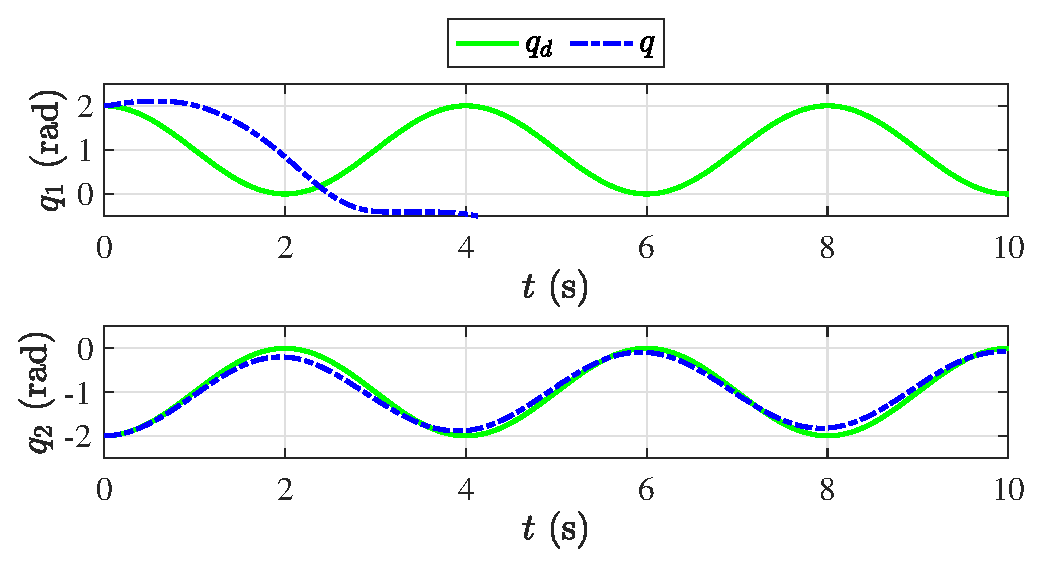
\includegraphics[width=0.49\linewidth]{imgs/Chap4/fig1.eps}%
%         \label{chap4:fig:track_CM1}}
%     \hfill
%         \subfloat[DNN-BSC]{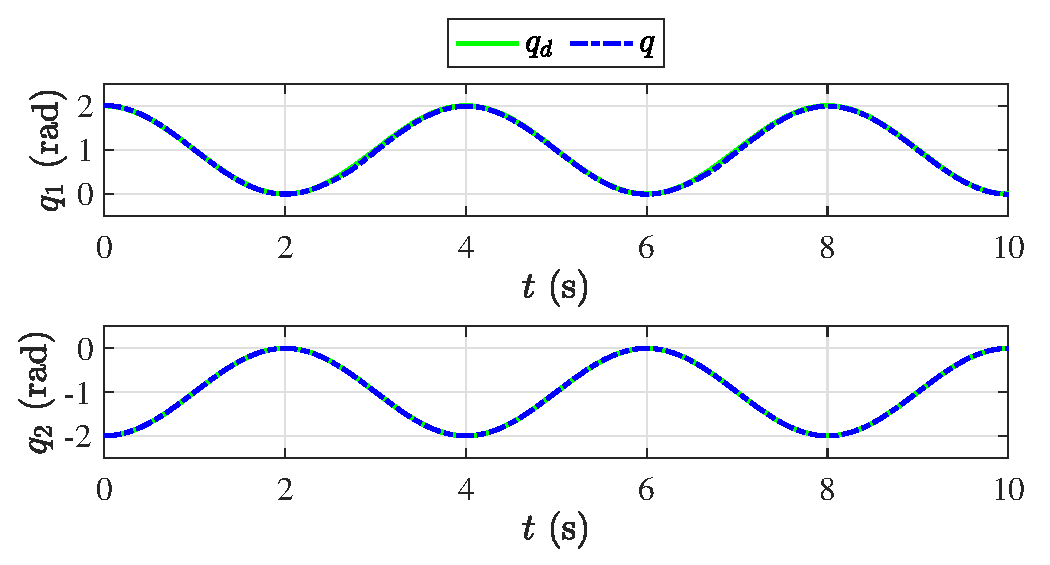
\includegraphics[width=0.49\linewidth]{imgs/Chap4/fig2.eps}%
%         \label{chap4:fig:track_CM2}}
%     \vfill
%         \subfloat[DNN-BSC-A]{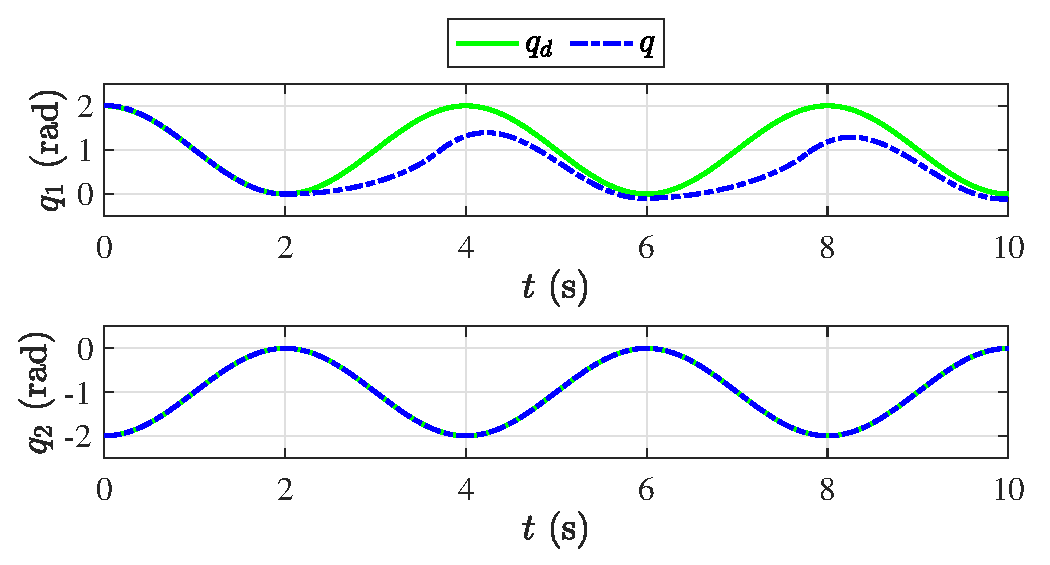
\includegraphics[width=0.49\linewidth]{imgs/Chap4/fig3.eps}%
%         \label{chap4:fig:track_CM3}}
%     \hfill
%         \subfloat[CoNAC]{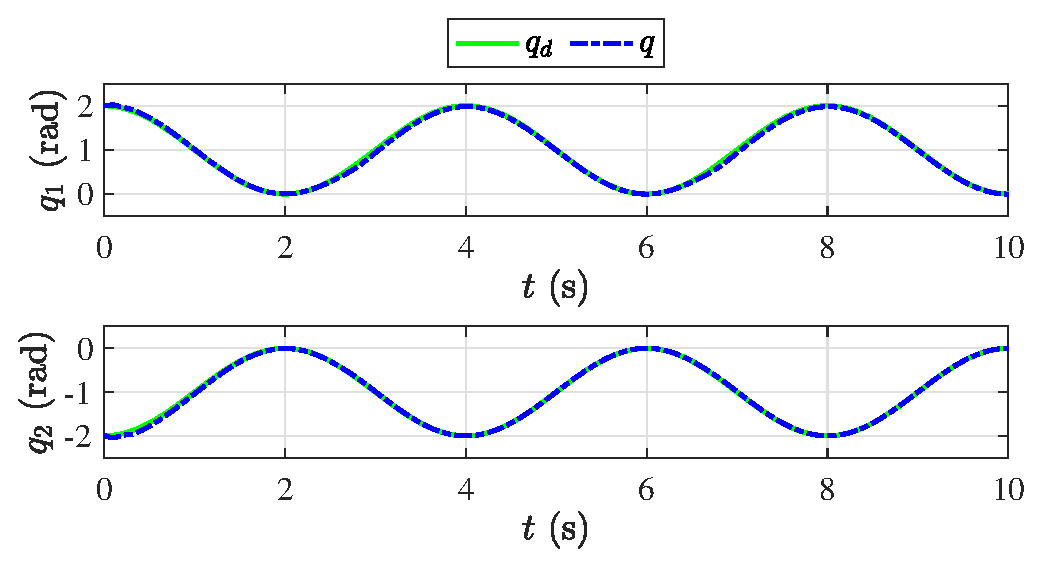
\includegraphics[width=0.49\linewidth]{imgs/Chap4/fig4.eps}%
%         \label{chap4:fig:track_CoNAC}}
%     \caption{Comparison of the tracking performance across the selected controllers.}
%     \label{chap4:fig:tracking}
% \end{figure}

\begin{figure}[!t]
    \centering
        \subfloat[BSC]{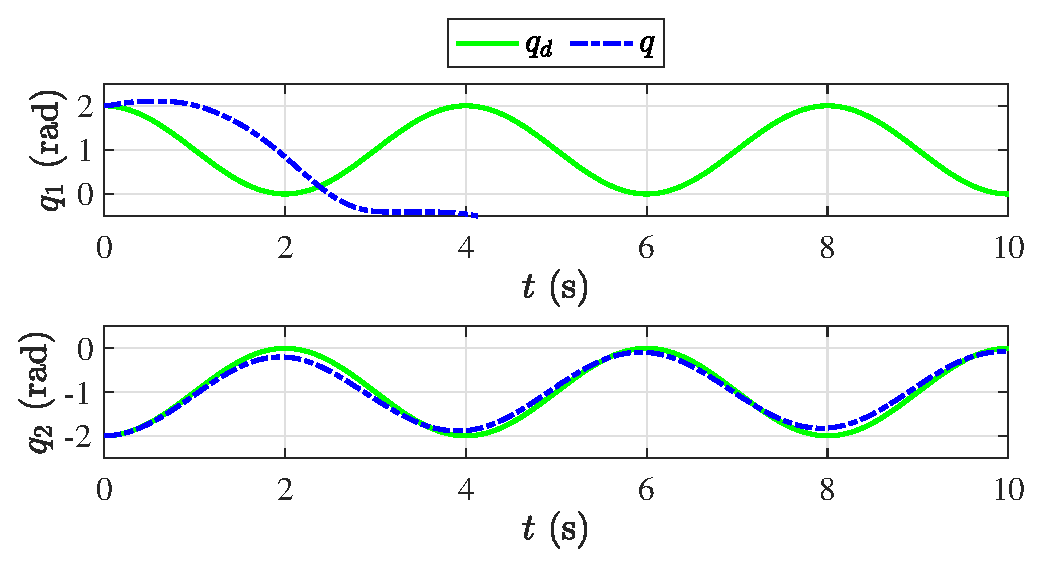
\includegraphics[width=0.8\linewidth]{imgs/Chap4/fig1.eps}%
        \label{chap4:fig:track_CM1}}
    \vfill
        \subfloat[DNN-BSC]{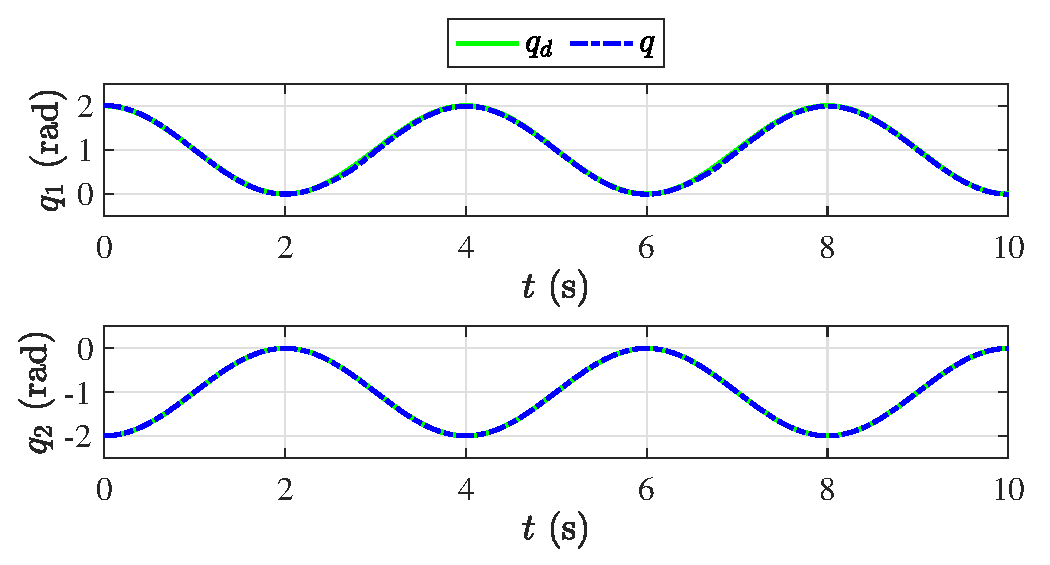
\includegraphics[width=0.8\linewidth]{imgs/Chap4/fig2.eps}%
        \label{chap4:fig:track_CM2}}
    \caption{Comparison of the tracking performance of BSC and DNN-BSC.}
    \label{chap4:fig:tracking1}
\end{figure}

\begin{figure}[!t]
    \centering
        \subfloat[DNN-BSC-A]{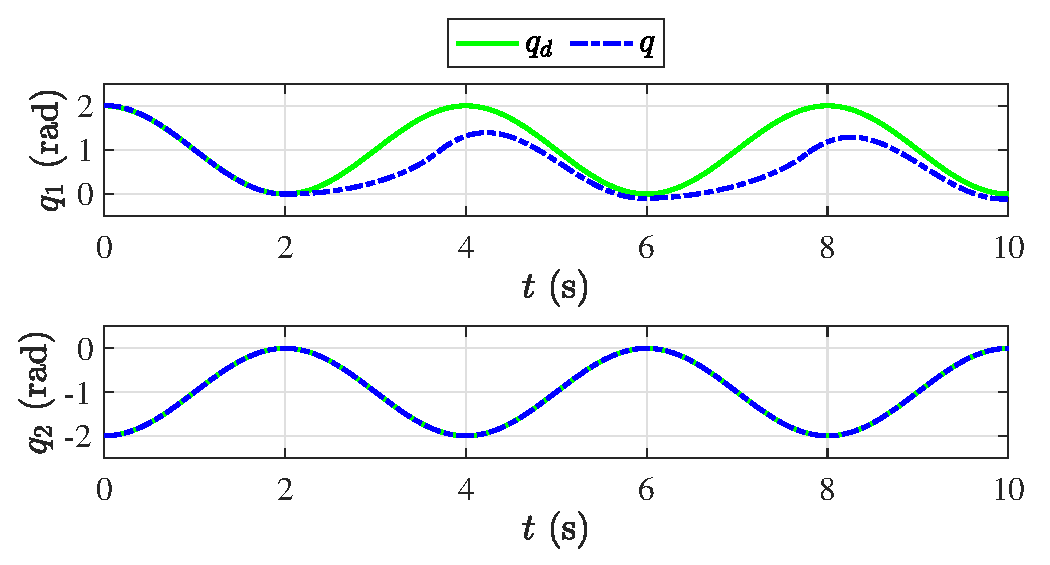
\includegraphics[width=0.8\linewidth]{imgs/Chap4/fig3.eps}%
        \label{chap4:fig:track_CM3}}
    \vfill
        \subfloat[CoNAC]{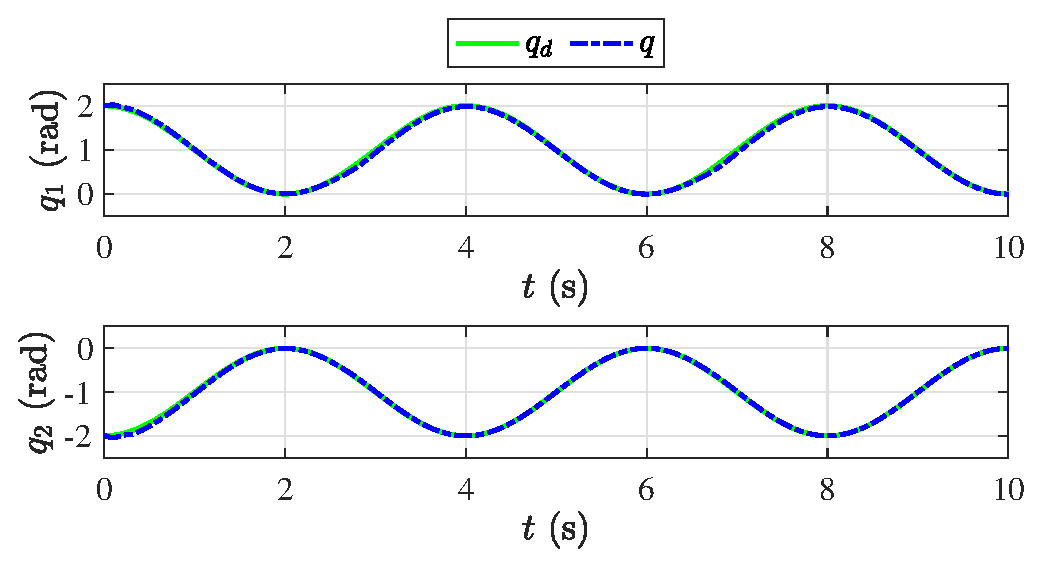
\includegraphics[width=0.8\linewidth]{imgs/Chap4/fig4.eps}%
        \label{chap4:fig:track_CoNAC}}
    \caption{Comparison of the tracking performance of DNN-BSC-A and CoNAC.}
    \label{chap4:fig:tracking2}
\end{figure}

% \begin{figure}[!t]
%     \centering
%         \subfloat[BSC]{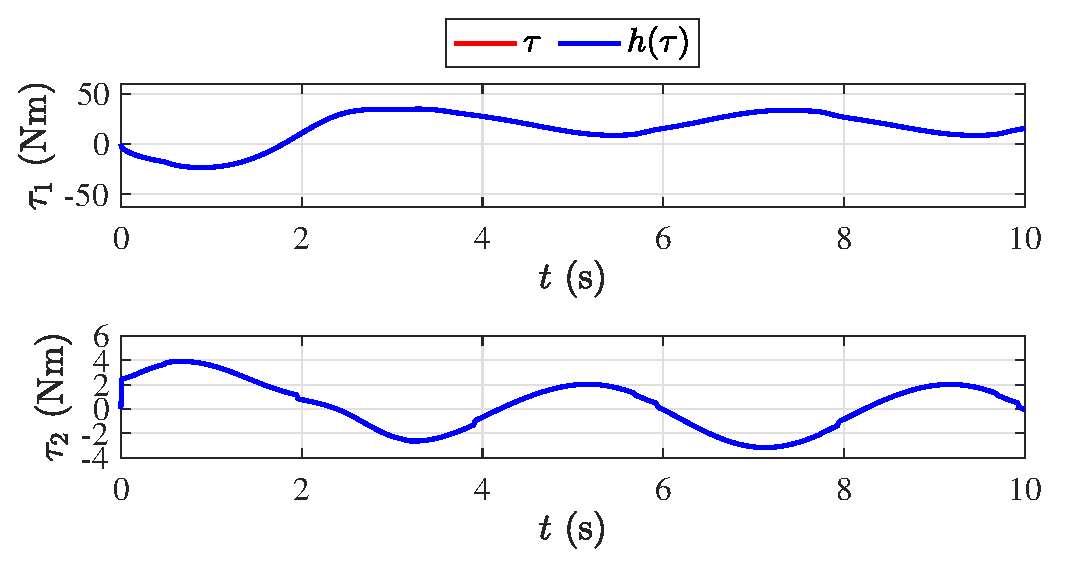
\includegraphics[width=0.49\linewidth]{imgs/Chap4/fig5.eps}%
%         \label{chap4:fig:control_CM1}}
%     \hfill
%         \subfloat[DNN-BSC]{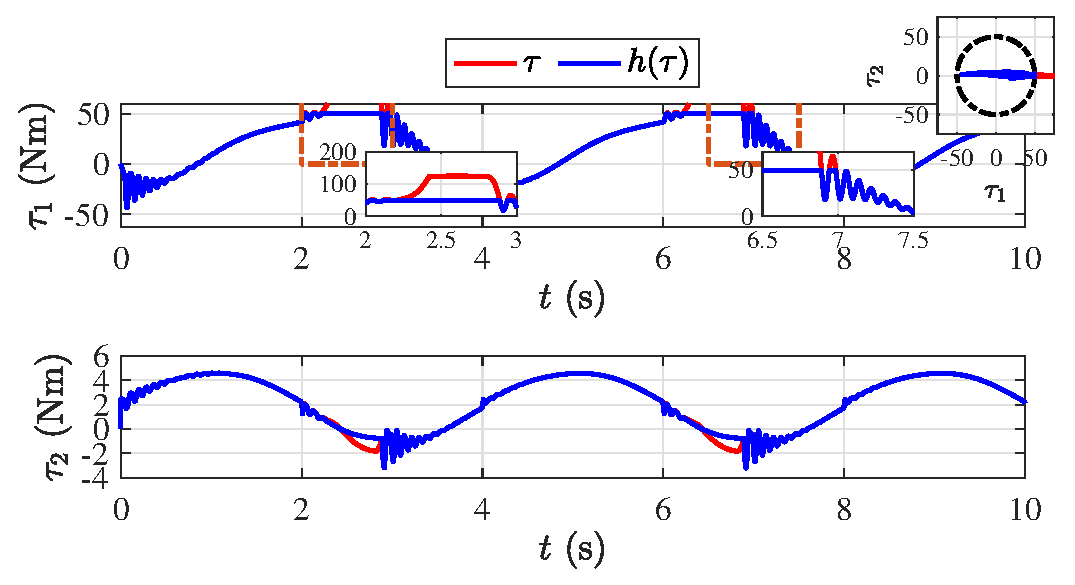
\includegraphics[width=0.49\linewidth]{imgs/Chap4/fig6.eps}%
%         \label{chap4:fig:control_CM2}}
%     \vfill
%         \subfloat[DNN-BSC-A]{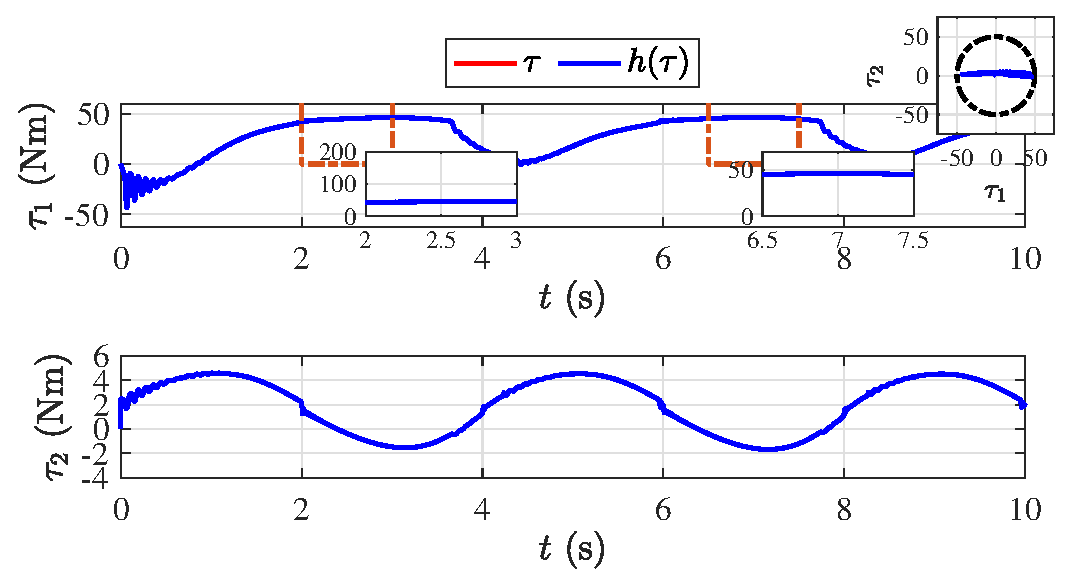
\includegraphics[width=0.49\linewidth]{imgs/Chap4/fig7.eps}%
%         \label{chap4:fig:control_CM3}}
%     \hfill
%         \subfloat[CoNAC]{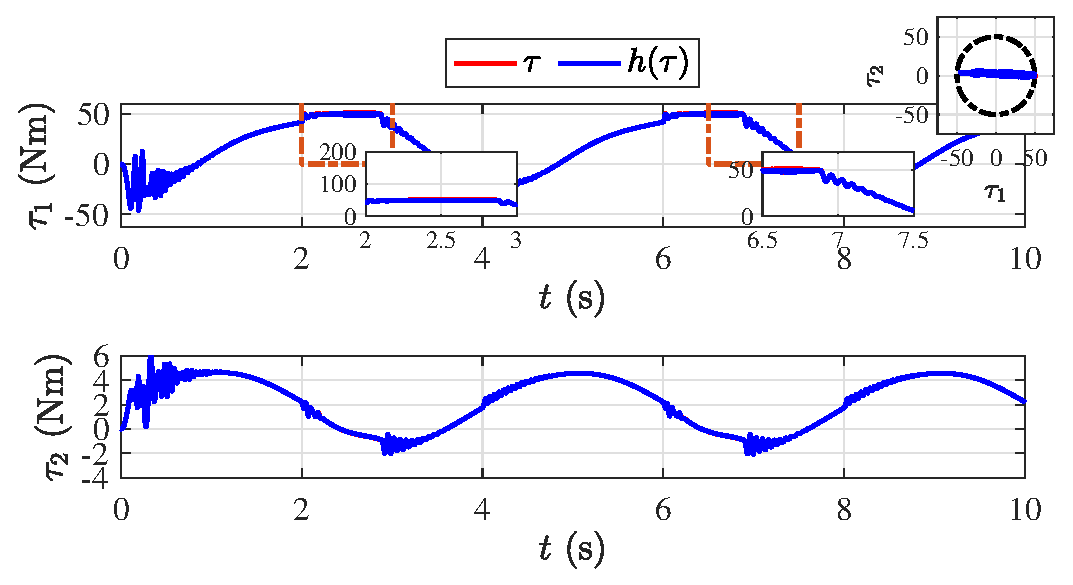
\includegraphics[width=0.49\linewidth]{imgs/Chap4/fig8.eps}%
%         \label{chap4:fig:control_CoNAC}}
%     \vfill
%     \caption{Comparison of the control input $\tau$ and the physically saturated control input $h(\tau)$ across the selected controllers.}
%     \label{chap4:fig:control}
% \end{figure}

\begin{figure}[!t]
    \centering
        \subfloat[BSC]{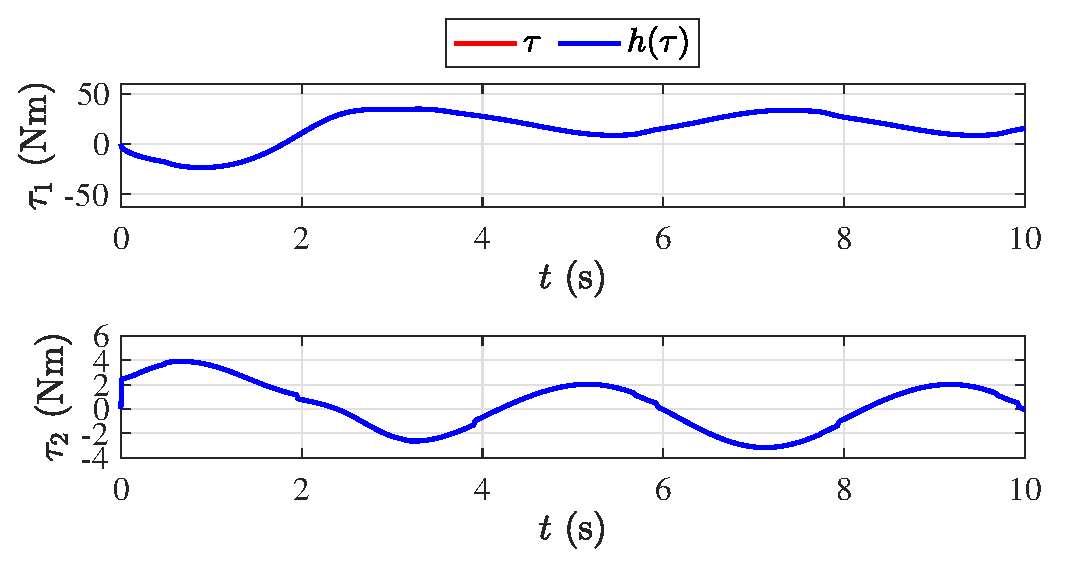
\includegraphics[width=0.8\linewidth]{imgs/Chap4/fig5.eps}%
        \label{chap4:fig:control_CM1}}
    \vfill
        \subfloat[DNN-BSC]{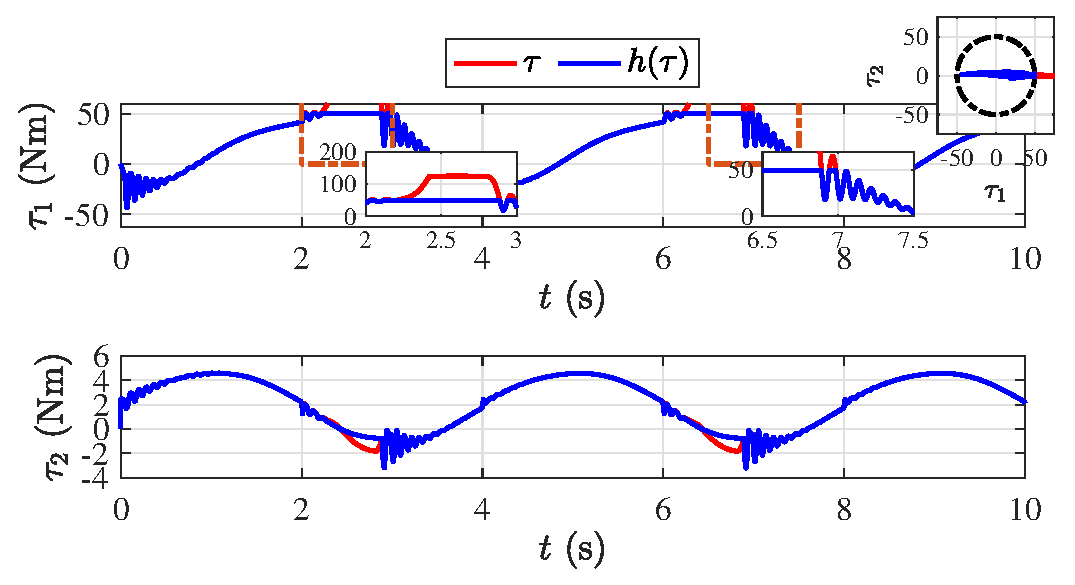
\includegraphics[width=0.8\linewidth]{imgs/Chap4/fig6.eps}%
        \label{chap4:fig:control_CM2}}
    \caption{Comparison of the control input $\tau$ and the physically saturated control input $h(\tau)$ of BSC and DNN-BSC.}
    \label{chap4:fig:control1}
\end{figure}

\begin{figure}[!t]
    \centering
        \subfloat[DNN-BSC-A]{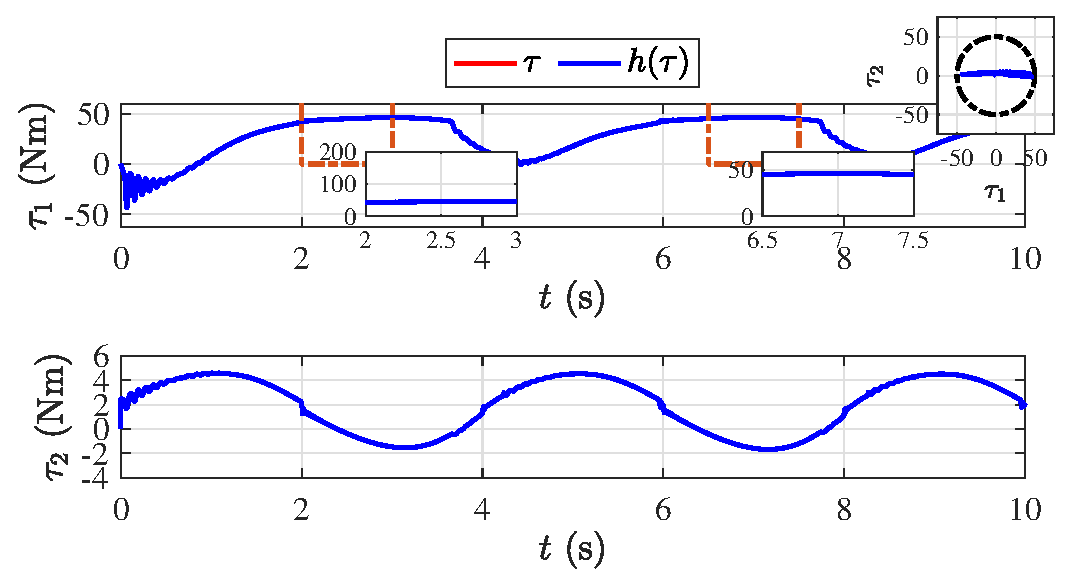
\includegraphics[width=0.8\linewidth]{imgs/Chap4/fig7.eps}%
        \label{chap4:fig:control_CM3}}
    \vfill
        \subfloat[CoNAC]{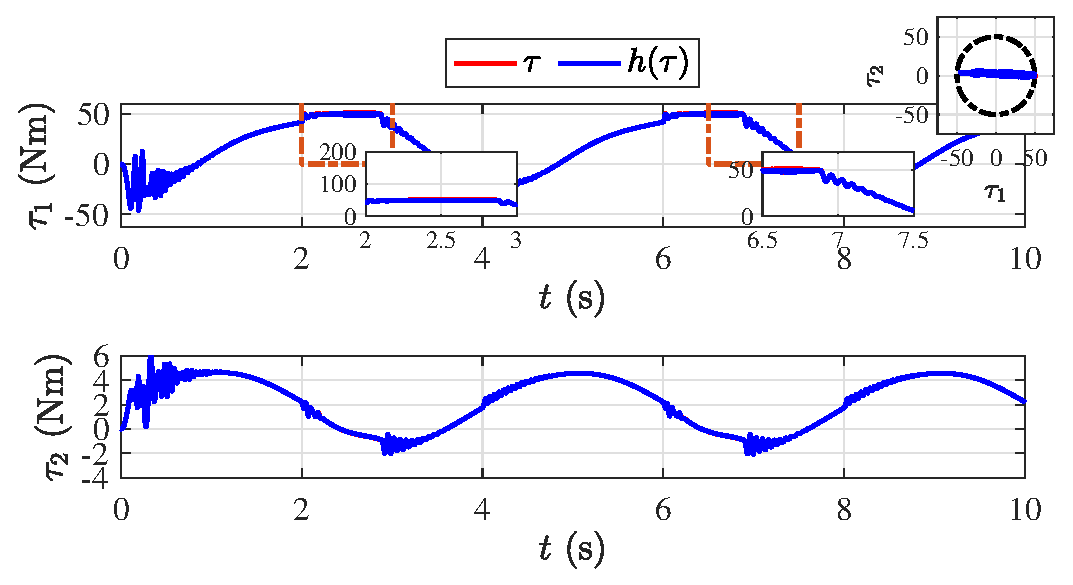
\includegraphics[width=0.8\linewidth]{imgs/Chap4/fig8.eps}%
        \label{chap4:fig:control_CoNAC}}
    \vfill
    \caption{Comparison of the control input $\tau$ and the physically saturated control input $h(\tau)$ of DNN-BSC-A and CoNAC.}
    \label{chap4:fig:control2}
\end{figure}

\begin{figure}[!t]
    \centering
    {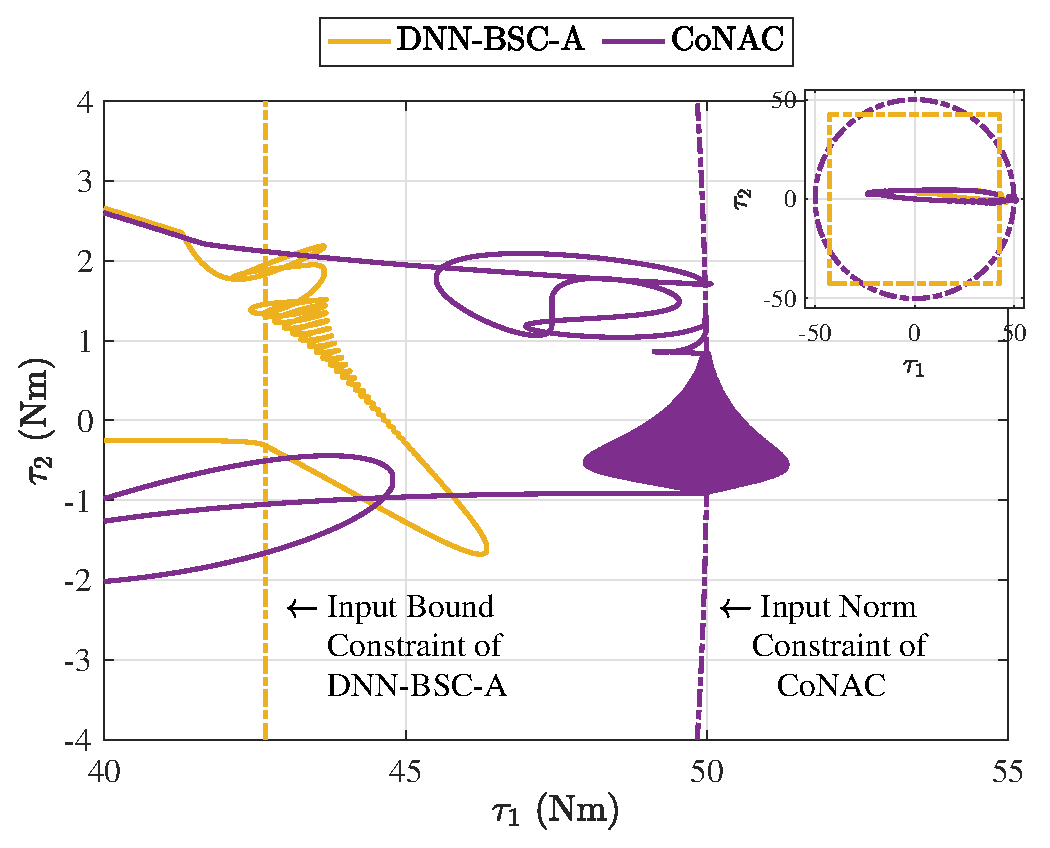
\includegraphics[width=0.85\linewidth]{imgs/Chap4/fig16.eps}
    \caption{Control input paths of DNN-BSC and CoNAC during the time interval from 5 s to 8 s.}
    \label{chap4:fig:control_ball}}
\end{figure}

% \begin{figure}[!t]
%     \centering
%         \subfloat[Multipliers of CoNAC]{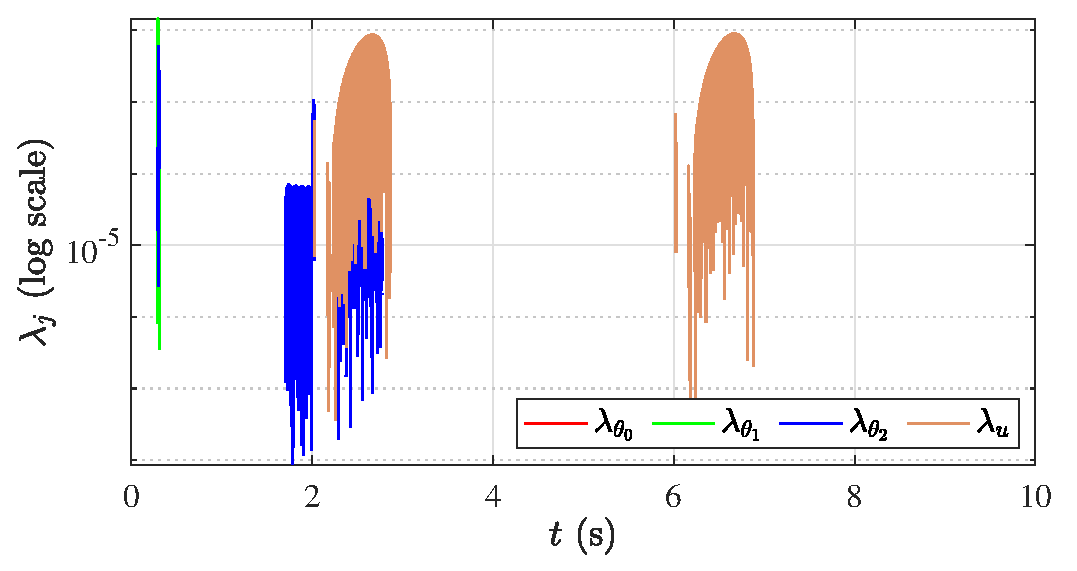
\includegraphics[width=0.49\linewidth]{imgs/Chap4/fig12.eps}%
%         \label{chap4:fig:multiplier}}
%     \hfill
%         \subfloat[Weight norms of DNN-BSC]{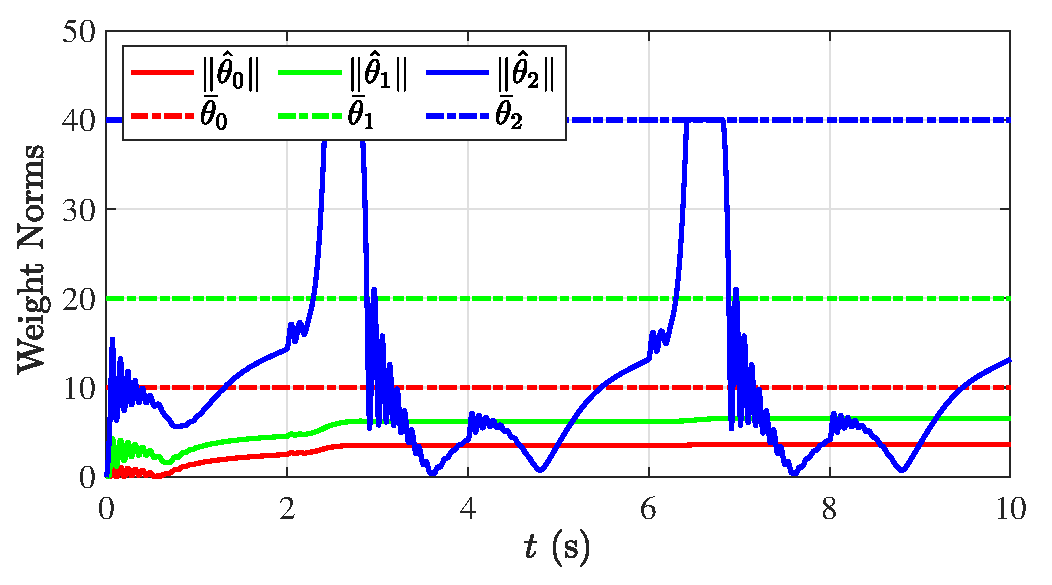
\includegraphics[width=0.49\linewidth]{imgs/Chap4/fig9.eps}%
%         \label{chap4:fig:weight_CM2}}
%     \vfill
%         \subfloat[Weight norms of DNN-BSC-A]{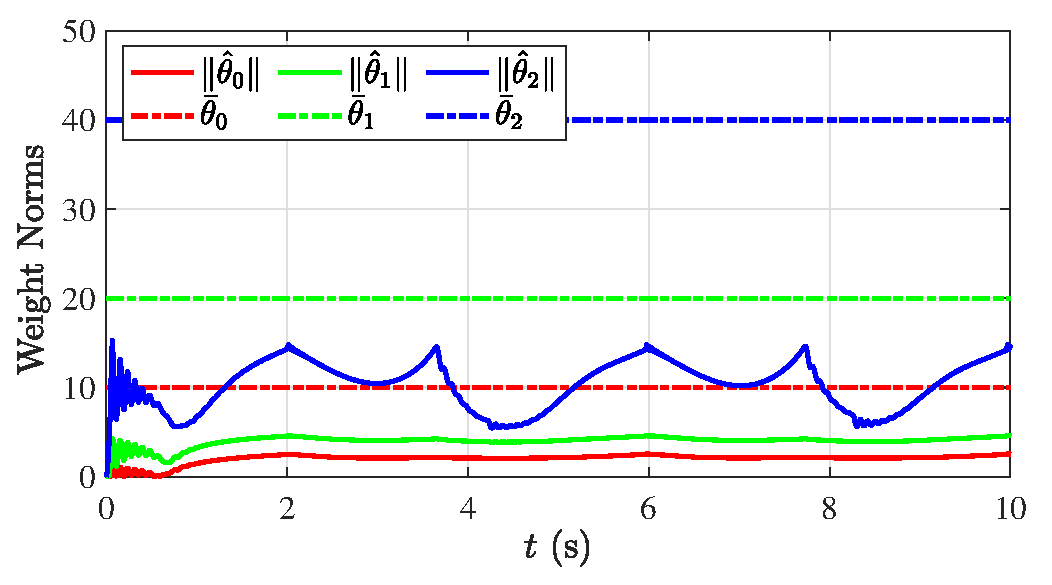
\includegraphics[width=0.49\linewidth]{imgs/Chap4/fig10.eps}%
%         \label{chap4:fig:weight_CM3}}
%     \hfill
%         \subfloat[Weight norms of CoNAC]{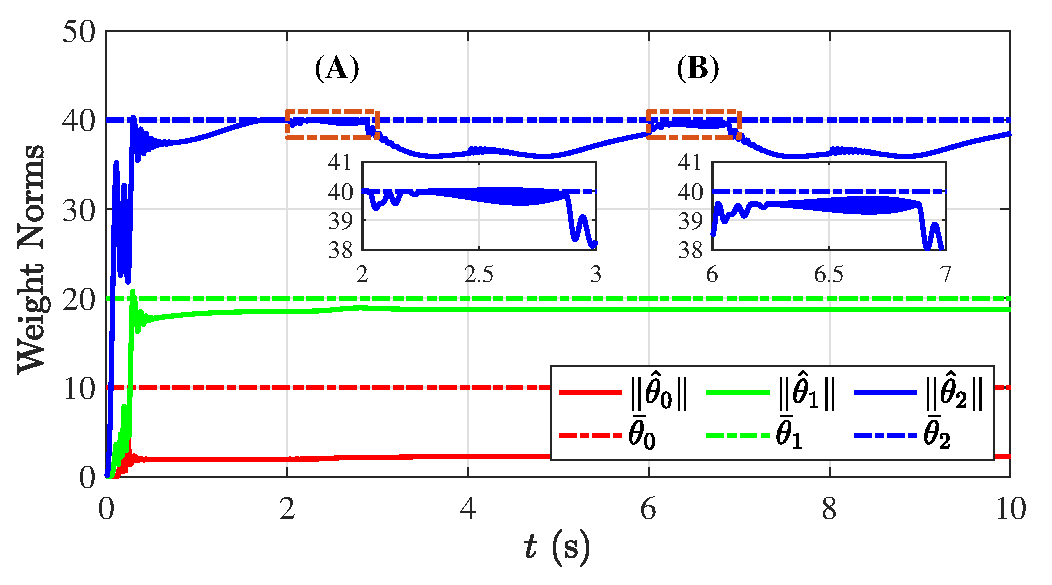
\includegraphics[width=0.49\linewidth]{imgs/Chap4/fig11.eps}%
%         \label{chap4:fig:weight_CoNAC}}       
%     \caption{Lagrange multipliers of CoNAC and weight norms of DNN-BSC, DNN-BSC-A, and CoNAC.}
%     \label{chap4:fig:weight_multiplier}
% \end{figure}

\begin{figure}[!t]
    \centering
        \subfloat[Weight norms of DNN-BSC]{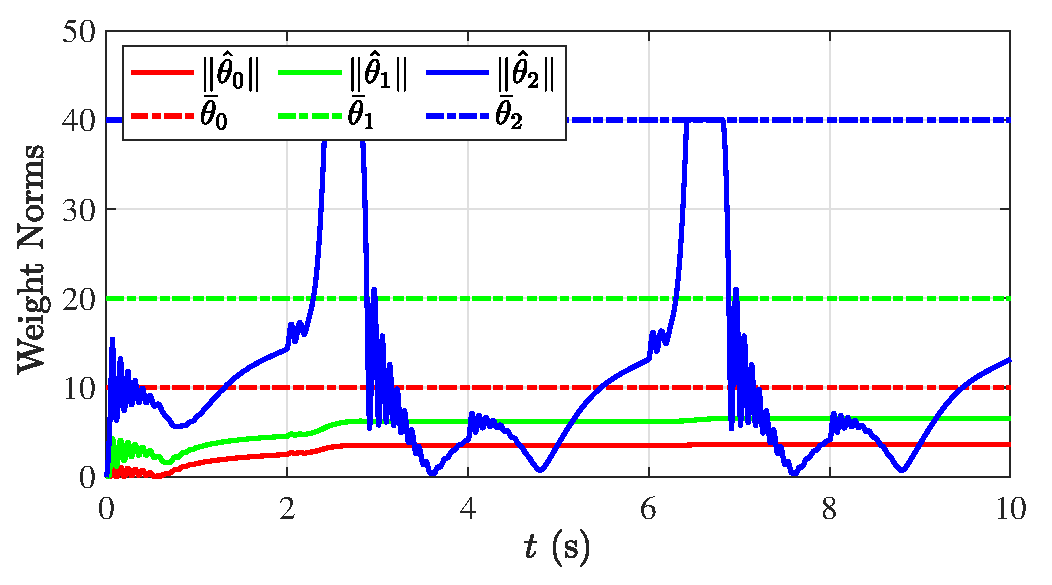
\includegraphics[width=0.8\linewidth]{imgs/Chap4/fig9.eps}%
        \label{chap4:fig:weight_CM2}}
    \vfill
        \subfloat[Weight norms of DNN-BSC-A]{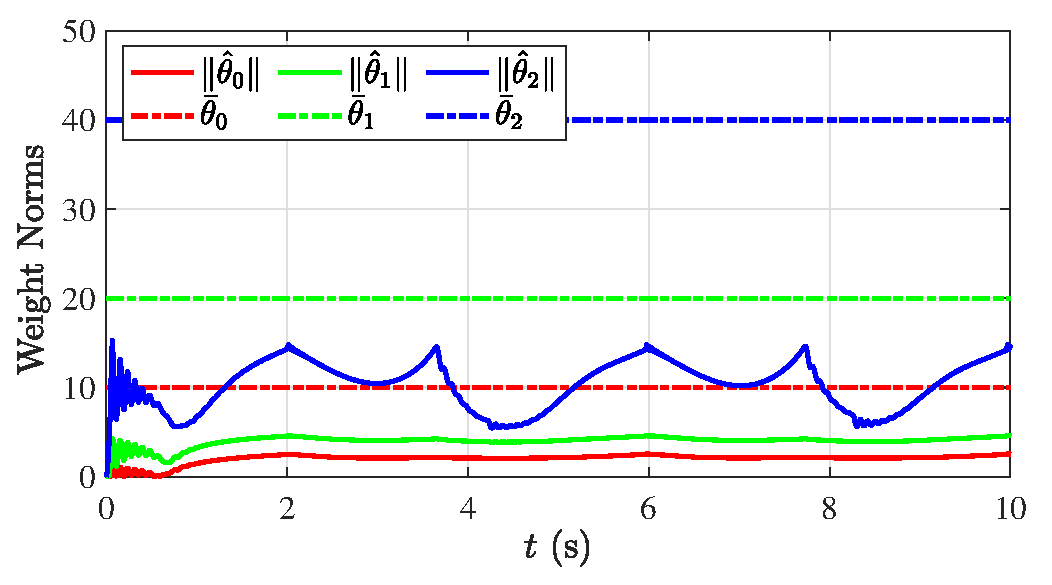
\includegraphics[width=0.8\linewidth]{imgs/Chap4/fig10.eps}%
        \label{chap4:fig:weight_CM3}}
    \caption{Weight norms of DNN-BSC and DNN-BSC-A.}
    \label{chap4:fig:weight_multiplier1}
\end{figure}

\begin{figure}[!t]
    \centering
        \subfloat[Multipliers of CoNAC]{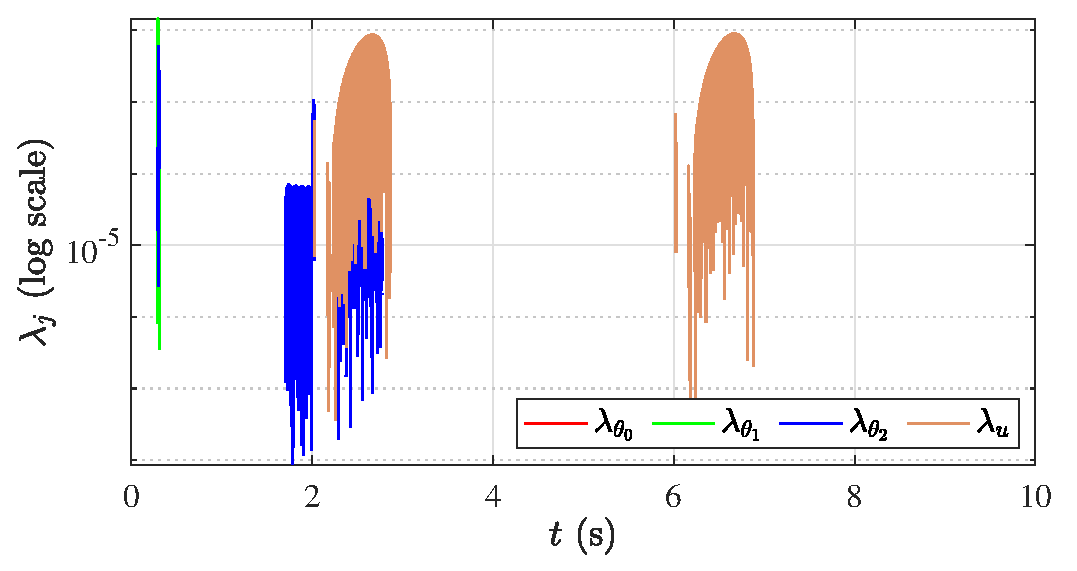
\includegraphics[width=0.8\linewidth]{imgs/Chap4/fig12.eps}%
        \label{chap4:fig:multiplier}}
    \vfill
        \subfloat[Weight norms of CoNAC]{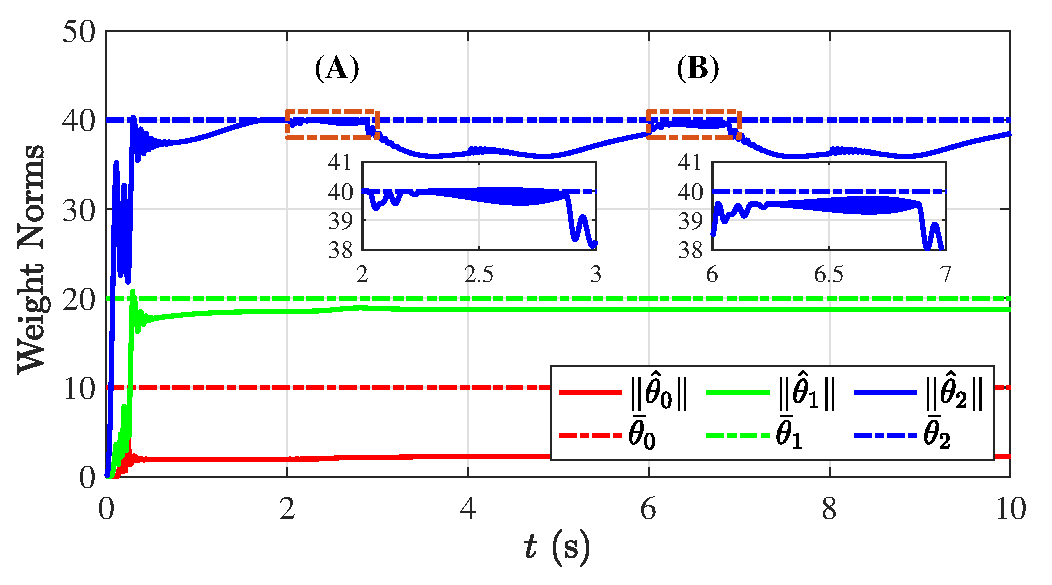
\includegraphics[width=0.8\linewidth]{imgs/Chap4/fig11.eps}%
        \label{chap4:fig:weight_CoNAC}}       
    \caption{Lagrange multipliers and weight norms CoNAC.}
    \label{chap4:fig:weight_multiplier2}
\end{figure}

% SIMULATION FIGURES
% **********************************************************

\subsection{Results}

\subsubsection{System Uncertainty Handling}

The tracking results of the selected controllers are shown in Fig.~\ref{chap4:fig:tracking1} and Fig.~\ref{chap4:fig:tracking2}.
To demonstrate the effectiveness of using DNNs for compensating the lumped system uncertainty function $f$, the gains ${k_q}$ and ${k_z}$ for BSC were intentionally selected as small values, resulting in a weak ability to handle these uncertainties. As a result,
%poor performance and sufficiently large values to satisfy \eqref{eq. ctrl stable condition}.
%the parameters of CM1 are poorly tuned, 
BSC failed to track the reference trajectory, as shown in Fig.~\ref{chap4:fig:track_CM1}.

By leveraging the DNN to compensate for the lumped system uncertainty within the BSC, DNN-BSC achieved improved tracking performance compared to BSC, as seen in Fig.~\ref{chap4:fig:track_CM2}. Fig.~\ref{chap4:fig:track_CM3} shows that DNN-BSC-A enhanced tracking performance for $q_2$, but tracking for $q_1$ remained unsatisfactory due to incomplete constraint handling, which will be discussed in detail in Section \ref{chap4:sec:sim:cstr input}.

Finally, CoNAC, which directly approximates the stabilizing control law along with the compensation term, demonstrated satisfactory tracking performance across both states, as illustrated in Fig.~\ref{chap4:fig:track_CoNAC}.

\subsubsection{Input Norm Constraint Handling} \label{chap4:sec:sim:cstr input}

The resulting control input $\tau$ and physically saturation control input $h(\tau)$ for the selected controllers are shown in Fig.~\ref{chap4:fig:control1} and Fig.~\ref{chap4:fig:control2}. As illustrated in Fig.~\ref{chap4:fig:control_CM1}, BSC did not violate the input norm constraint (\ie $\tau = h(\tau)$). However, in DNN-BSC, the added compensation term from the DNN caused violations of the input norm constraint (\ie $\tau > h(\tau)$) at several points; see Fig.~\ref{chap4:fig:control_CM2}. This failure to account for the input norm constraint led to oscillations in the control input $\tau$. The DNN adaptation process attempted to increase the weights to reduce the residual errors that were not constrained by saturation, but after saturation ceased, the control input had to rapidly adjust back to realistic levels, leading to oscillatory behavior. Such high-frequency oscillations may induce instability in the control system or cause fatigue in the actuators.

On the other hand, both DNN-BSC-A and CoNAC successfully handled their imposed input constraints, as shown in Fig.~\ref{chap4:fig:control_CM3} and Fig.~\ref{chap4:fig:control_CoNAC}, respectively, without causing notable oscillations in the control input $\tau$ even after the input constraint was activated. However, the tracking performance of DNN-BSC-A was lower than that of DNN-BSC and CoNAC, as the auxiliary system used in DNN-BSC-A approximated the input norm constraint with an input bound constraint, creating a rectangular constraint in the $\tau$-space (see Fig.~\ref{chap4:fig:control_ball}). In contrast, CoNAC satisfied the nonlinear input norm constraint and produced the physically maximum control input, resulting in improved tracking performance. 

It is also important to note that the control input trajectory in DNN-BSC-A depends on the dynamics of the auxiliary system. The auxiliary system regulates the violated control input after sufficient auxiliary state $\zeta$ is generated to compensate for the violation. This can be observed in Fig.~\ref{chap4:fig:control_ball}, where DNN-BSC-A exhibited minor violations of the input bound constraint. In contrast, CoNAC satisfied the constraint without being affected by such dynamics, as its Lagrange multiplier adjusted as soon as the constraint was violated.

\subsubsection{Weight Norm Constraint Handling}

The resulting weight norms of DNN-BSC, DNN-BSC-A, and CoNAC, along with the Lagrange multipliers of CoNAC, are shown in Fig.~\ref{chap4:fig:weight_multiplier1} and Fig.~\ref{chap4:fig:weight_multiplier2}. All three controllers—DNN-BSC, DNN-BSC-A, and CoNAC—maintained weight norms within the imposed weight norm constraints.

IN DNN-BSC, as shown in Fig.~\ref{chap4:fig:weight_CM2}, the weight norm of the last layer (\ie $\Vert {{{\hat \theta }_2}} \Vert$) fluctuated significantly over time, proportional to the control input norm. This is because the last layer’s weights directly determine the control input. When the control input violated the input norm constraint, the last layer’s weight norm hit the boundary and stayed there due to the projection operator. However, the projection operator only responded to violations without considering optimality or behavior.
%In the case of CM2 which does not consider the control input constraint, the weight norm of the last layer reaches the maximum weight norm value, when the control is saturated.
%It is because the weights get increased to produce larger control input to reduce the tracking error of $q_2$. (\ie the maximum magnitude of the control input depends on the weight norm of the last layer, since the activation function is bounded.)

In DNN-BSC-A, none of the weight norms reached their boundaries, as shown in Fig.~\ref{chap4:fig:weight_CM3}. This was due to the auxiliary system, where the auxiliary state $\zeta$ reduced the control input, ensuring it stayed within the input constraint.

In CoNAC, all weight norms complied with the imposed constraints through the constrained optimization approach, as illustrated in Fig.\ref{chap4:fig:weight_CoNAC}. When any weight norm approached its upper limit, the Lagrange multiplier was promptly activated to steer the weight adaptation direction towards a constraint-satisfactory point (see Fig.\ref{chap4:fig:multiplier}). Notably, the weight norms of the first and second layers ($\Vert {{{\hat \theta }_0}} \Vert$ and $\Vert {{{\hat \theta }_1}} \Vert$) remained nearly constant throughout the control period. The weight norm of the last layer $\Vert {{{\hat \theta }_2}} \Vert$ stabilized within the upper bound by around 6.5 seconds (see Fig.~\ref{chap4:fig:weight_CoNAC} (B)), coinciding with the activation of the input norm constraint. This quasi-static behavior of the weight norm (\ie $d{\hat\theta}/dt=-\alpha\partial L/\partial \hat\theta \approx 0$) along with the quasi-static behavior of the Lagrange multipliers (\ie $\dot\lambda_j = \beta_j c_j \approx 0$) implies that the weights were updated near the KKT conditions, signifying local optimality in CoNAC. However, at around 2.5 seconds (see Fig.~\ref{chap4:fig:weight_CoNAC} (A)), the weight norm of the last layer reached the upper limit earlier, despite similar control conditions as the case at 6.5 seconds. This earlier saturation likely occurred because the optimization process had not yet fully converged to the optimal weight values.

The overall weight norms of CoNAC were larger than those of DNN-BSC and DNN-BSC-A, since CoNAC approximated the entire stabilizing control law, whereas DNN-BSC and DNN-BSC-A only approximated the system uncertainty term within the BSC framework.

\subsubsection{Comparison Analysis of Computation Times}

\begin{table}[!t]
    \renewcommand{\arraystretch}{1.3}
    \caption{Average computation times.}
    \centering
    \begin{tabular}{|c||c|c|c|c|c|}
    \hline
    Computation time & \textbf{BSC} & \textbf{DNN-BSC} & \textbf{DNN-BSC-A} & \textbf{CoNAC} \\
    \hline 
    Control ($10^{-5}$~s) & 0.087 & 0.755 & 0.7477 & 0.7465 \\
    \hline
    Ratio & 0.112 & 1 & 0.988 & 0.987 \\
    \hline
    Train ($\times 10^{-5}$~s) & - & 3.877 & 3.821 & 3.826 \\
    \hline
    Ratio & - & 1 &∆ 0.986 & 0.987 \\ 
    \hline
    \end{tabular}
    \label{chap4:table:comp_time}
\end{table}

In addition, the computation times were analyzed and summarized in Table \ref{chap4:table:comp_time}.
The MATLAB's functions \texttt{tic} and \texttt{toc} were used to measure the computation time at each time step and the average values were calculated.
The simulations were conducted on a MacBook Air (2021 model) with an M1 processor and 8 GB of RAM.
The computation times of DNN-BSC were used as the reference for the comparison.

The computing times of the control decisions and training processes of all controllers were below the simulation sampling time $T_s=10^{-4}$ indicating their suitability for real-time applications, as shown in Table \ref{chap4:table:comp_time}.
Notably, controllers utilizing DNNs exhibited higher computation times than BSC due to the additional processing required for the DNNs.
However, compared to the DNN-BSC and DNN-BSC-A, the CoNAC had similar computation times for both the control and training processes.
In other words, even though the CoNAC involves the additional process for the constraints and the Lagrange multipliers, its computation times were not significantly increased compared to the DNN-BSC and DNN-BSC-A.
Therefore, the CoNAC can achieve the better tracking performance and the constraint handling capability which were discussed in aforementioned sections, without notable increase in the computation times compared to existing methods with DNNs.  

%%%%%%%%%%%%%%%%%%%%%%%%%%%%%%%%
\section{Conclusion} 
%%%%%%%%%%%%%%%%%%%%%%%%%%%%%%%%

In this chapter, a constrained optimization-based neuro-adaptive controller (CoN\allowbreak AC) for the uncertain Euler-Lagrange system is extended to address both weight norm and input constraints using deep neural network (DNN).
The adaptation law is derived through a rigorous optimization framework. 
The stability of the proposed controller was analyzed using Lyapunov theory, ensuring that the system maintains bounded tracking and estimation errors under real-time adaptation.

The controller effectively incorporated both the input (bound or norm) constraint and the weight norm constraint, ensuring that both actuator limitations and neural network weights were kept within predefined bounds. 
By formulating these constraints as part of the optimization process, CoNAC ensured that the weights converged in a way that satisfied the Karush-Kuhn-Tucker (KKT) conditions, guaranteeing optimality and stability.

Simulation results validated the superior performance of CoNAC compared to conventional methods, such as DNN-BSC and DNN-BSC-A. 
CoNAC not only handled complex input constraints but also managed the weight norm constraints rigorously, leading to improved tracking accuracy and stability without notable oscillations.
